%% 
%% Copyright 2007-2020 Elsevier Ltd
%% 
%% This file is part of the 'Elsarticle Bundle'.
%% ---------------------------------------------
%% 
%% It may be distributed under the conditions of the LaTeX Project Public
%% License, either version 1.2 of this license or (at your option) any
%% later version.  The latest version of this license is in
%%    http://www.latex-project.org/lppl.txt
%% and version 1.2 or later is part of all distributions of LaTeX
%% version 1999/12/01 or later.
%% 
%% The list of all files belonging to the 'Elsarticle Bundle' is
%% given in the file `manifest.txt'.
%% 
%% Template article for Elsevier's document class `elsarticle'
%% with harvard style bibliographic references

\documentclass[preprint,12pt,authoryear]{elsarticle}

%% Use the option review to obtain double line spacing
%% \documentclass[authoryear,preprint,review,12pt]{elsarticle}

%% Use the options 1p,twocolumn; 3p; 3p,twocolumn; 5p; or 5p,twocolumn
%% for a journal layout:
%% \documentclass[final,1p,times,authoryear]{elsarticle}
%% \documentclass[final,1p,times,twocolumn,authoryear]{elsarticle}
%% \documentclass[final,3p,times,authoryear]{elsarticle}
%% \documentclass[final,3p,times,twocolumn,authoryear]{elsarticle}
%% \documentclass[final,5p,times,authoryear]{elsarticle}
%% \documentclass[final,5p,times,twocolumn,authoryear]{elsarticle}

%% For including figures, graphicx.sty has been loaded in
%% elsarticle.cls. If you prefer to use the old commands
%% please give \usepackage{epsfig}

%% The amssymb package provides various useful mathematical symbols
\usepackage{amssymb}
%% The amsthm package provides extended theorem environments
%% \usepackage{amsthm}

%% The lineno packages adds line numbers. Start line numbering with
%% \begin{linenumbers}, end it with \end{linenumbers}. Or switch it on
%% for the whole article with \linenumbers.
%% \usepackage{lineno}

\usepackage{hyperref}
\usepackage{tikz}
\usetikzlibrary{mindmap}
\usepackage{multirow}
\usepackage{pgfplots}
\usepackage{arydshln}

\journal{Academic Radiology}

\pgfplotsset{compat=1.13}

\begin{document}

\begin{frontmatter}

%% Title, authors and addresses

%% use the tnoteref command within \title for footnotes;
%% use the tnotetext command for theassociated footnote;
%% use the fnref command within \author or \affiliation for footnotes;
%% use the fntext command for theassociated footnote;
%% use the corref command within \author for corresponding author footnotes;
%% use the cortext command for theassociated footnote;
%% use the ead command for the email address,
%% and the form \ead[url] for the home page:
%% \title{Title\tnoteref{label1}}
%% \tnotetext[label1]{}
%% \author{Name\corref{cor1}\fnref{label2}}
%% \ead{email address}
%% \ead[url]{home page}
%% \fntext[label2]{}
%% \cortext[cor1]{}
%% \affiliation{organization={},
%%            addressline={}, 
%%            city={},
%%            postcode={}, 
%%            state={},
%%            country={}}
%% \fntext[label3]{}

\title{State of the Practice for Medical Imaging Software}

%% use optional labels to link authors explicitly to addresses:
%% \author[label1,label2]{}
%% \affiliation[label1]{organization={},
%%             addressline={},
%%             city={},
%%             postcode={},
%%             state={},
%%             country={}}
%%
%% \affiliation[label2]{organization={},
%%             addressline={},
%%             city={},
%%             postcode={},
%%             state={},
%%             country={}}

\author[CAS]{Spencer Smith}
\author[CAS]{Ao Dong}
\author[CAS]{Jacques Carette}
\author[ECE]{Mike Noseworthy}

\affiliation[CAS]{organization={McMaster University, Computing and Software Department},%Department and Organization
            addressline={1280 Main Street West}, 
            city={Hamilton},
            postcode={L8S 4K1}, 
            state={Ontario},
            country={Canada}}

\affiliation[ECE]{organization={McMaster University, Electrical Engineering},%Department and Organization
            addressline={1280 Main Street West}, 
            city={Hamilton},
            postcode={L8S 4K1}, 
            state={Ontario},
            country={Canada}}

\begin{abstract}

We present a general method to assess the state of the practice for Scientific
Computing (SC) software and apply this method to Medical Imaging (MI) software.
We selected 29 MI software projects from 48 candidates, assessed 10 software
qualities (installability, correctness/ verifiability, reliability, robustness,
usability, maintainability, reusability, understandability,
visibility/transparency and reproducibility) by answering 103 questions for each
software project, and interviewed 8 of the 29 development teams. Based on the
quantitative data for the first 9 qualities, we ranked the MI software with the
Analytic Hierarchy Process (AHP). The top three software products were
\textit{3D Slicer}, \textit{ImageJ}, and \textit{OHIF Viewer}. By interviewing
the developers, we identified three major pain points: i) lack of resources; ii)
difficulty balancing between compatibility, maintainability, performance, and
security; and, iii) lack of access to real-world datasets for testing. For
future MI software projects, we propose adopting test-driven development, using
continuous integration and continuous delivery (CI/CD), using git and GitHub,
maintaining good documentation, supporting third-party plugins or extensions,
considering web application solutions, and improving collaboration between
different MI software projects.

\end{abstract}

%%Graphical abstract
%\begin{graphicalabstract}
%\includegraphics{grabs}
%\end{graphicalabstract}

%%Research highlights
%\begin{highlights}
%\item Research highlight 1
%\item Research highlight 2
%\end{highlights}

\begin{keyword}
	medical imaging, scientific computing, software engineering, software
	quality, Analytic Hierarchy Process, developer interviews
\end{keyword}

\end{frontmatter}

%% \linenumbers

\section{Introduction} \label{ch_intro}

We aim to study the state of software development practice for Medical Imaging
(MI) software.  MI tools use images of the interior of the body (from sources
such as Magnetic Resonance Imaging (MRI), Computed Tomography (CT), Positron
Emission Tomography (PET) and Ultrasound) to provide information for diagnostic,
analytic, and medical applications \citep{FDA2021, enwiki:1034887445,
Zhang2008}.  Given the importance of MI software and the high number of
competing software projects, we wish to understand the merits and drawbacks of
the current development processes, tools and methodologies.  We aim to assess
through a software engineering lens the quality of the existing software with
the hope of highlighting standout examples, understanding current pain points
and providing guidelines and recommendations for future development.

\subsection{Purpose} \label{sec_motivation}

Not only do we wish to gain insight into the state of the practice for MI
software, we also wish to understand the development of research software in
general. We wish to understand the impact of the often cited gap, or chasm,
between software engineering and scientific programming \citep{Storer2017}.
Although scientists spend a substantial proportion of their working hours on
software development \citep{Hannay2009, Prabhu2011}, many developers learn
software engineering skills by themselves or from their peers, instead of from
proper training \citep{Hannay2009}. \citet{Hannay2009} observe that many
scientists showed ignorance and indifference to standard software engineering
concepts. For instance, according to a survey by \citet{Prabhu2011}, more than
half of their 114 subjects did not use any proper debugger for their software.

To gain insights, we devised five research questions, which can be applied
to MI, and to other domains, of research software \citep{SmithEtAl2021}:

\begin{description}

\item[RQ1.] \hypertarget{rq1}What artifacts are present in current software
projects? What role does documentation play in the projects? What are the
developers' attitude toward it?
\item[RQ2.] \hypertarget{rq2}What tools are used in the development of current
software packages?
\item[RQ3.] \hypertarget{rq3}What principles, processes, and methodologies are
used in the development of current software packages?
\item[RQ4.] \hypertarget{rq4}What are the pain points for developers working on
research software projects? What aspects of the existing processes,
methodologies, and tools do they consider as potentially needing improvement?
What changes to processes, methodologies, and tools can improve software
development and software quality?
\item[RQ5.] \hypertarget{rq5}What is the current status of the following
software qualities for the projects? What actions have the developers taken to
address them?
\begin{itemize}
	\item Installability
	\item Correctness \& Verifiability
	\item Reliability
	\item Robustness
	\item Usability
	\item Maintainability
	\item Reusability
	\item Understandability
	\item Visibility/Transparency
	\item Reproducibility
\end{itemize}
\item[RQ6.] \hypertarget{rq6}How does software designated as high quality by
this methodology compare with top-rated software by the community?
\end{description}

\subsection{Overview of the Methodology}

We designed a general methodology to assess the state of the practice for SC
software \citep{SmithEtAl2021}. Details can be found in Section~\ref{}.  This
methodology builds off prior work to assess the state of the practice for such
domains as Geographic Information Systems \citep{smith2018state}, Mesh
Generators \citep{smith2016state}, Seismology software
\citep{Smith2018Seismology}, and Statistical software for psychology
\citep{smith2018statistical}.  In keeping with the previous methodology, we have
maintained the constraint that the work load for measuring a given domain should
be feasible for a team as small as one person, and for a short time,
ideally around a person month of effort. A person month is considered to be $20$
working days ($4$ weeks in a month, with $5$ days of work per week) at $8$
person hours per day, or $20 \cdot 8 = 160$ person hours.

With our methodology, we first choose an SC domain (in the current case MI) and
identify a list of about 30 software packages. We approximately measure the
qualities of each package by filling in a grading template (forward ref?).
Compared with our previous methodology, the new methodology also includes
repository based metrics, such as the number of files, number of lines of code,
percentage of issues that are closed, etc. (forward ref?).  With the
quantitative data in the grading template, we rank the software with the
Analytic Hierarchy Process (AHP) (forward ref?). After this, as another addition
to our previous methodology, we interview some of the development teams to
further understand the status of their development process (forward ref?).
Finally, we summarize the results and propose recommendations for future SC
software development (forward ref?).

\subsection{Scope} \label{sec_scope}

We need to restrict the scope of MI software that we consider so that the
measurement exercise is feasible within a person month of effort. MI considers a
broad range of different problems.  According to \citet{Bankman2000}, MI
software deals with six different basic problems, while \citet{Angenent2006}
pointed out that four fundamental problems are solved by MI software. While both
mentioned Segmentation, Registration, and Visualization of medical images,
Bankman also included Enhancement, Quantification, and three functions for MI
archiving and telemedicine systems (Compression, Storage, and Communication)
\citep{Bankman2000}. On the other hand, \citet{Angenent2006} included
Simulation. According to Wikipedia contributors \citep{enwiki:1034877594}, MI
software has primary functions in Segmentation, Registration, Visualization
(including the basic display, reformatted views, and 3D volume rendering),
Statistical Analysis, and Image-based Physiological Modelling. As
\citet{Kim2011} describes, the general steps of medical image analysis after
obtaining digital data include Enhancement, Segmentation, Feature Extraction,
Classification, and Interpretation. Besides the above major functions, some MI
software provides supportive functions. For example, with Tool Kit libraries VTK
\citep{SchroederEtAl2006} and ITK \citep{McCormick2014}, developers build
software with Visualization and Analysis functions; Picture Archiving and
Communication System (PACS) helps users to economically store and conveniently
access images \citep{Choplin1992}. 

Based on our literature survey, we divided MI software into five sub-groups and
several sub-sub-groups by their major functions, as shown in Figure
\ref{fig_mi_functions}.

\begin{figure}[ht]
\centering
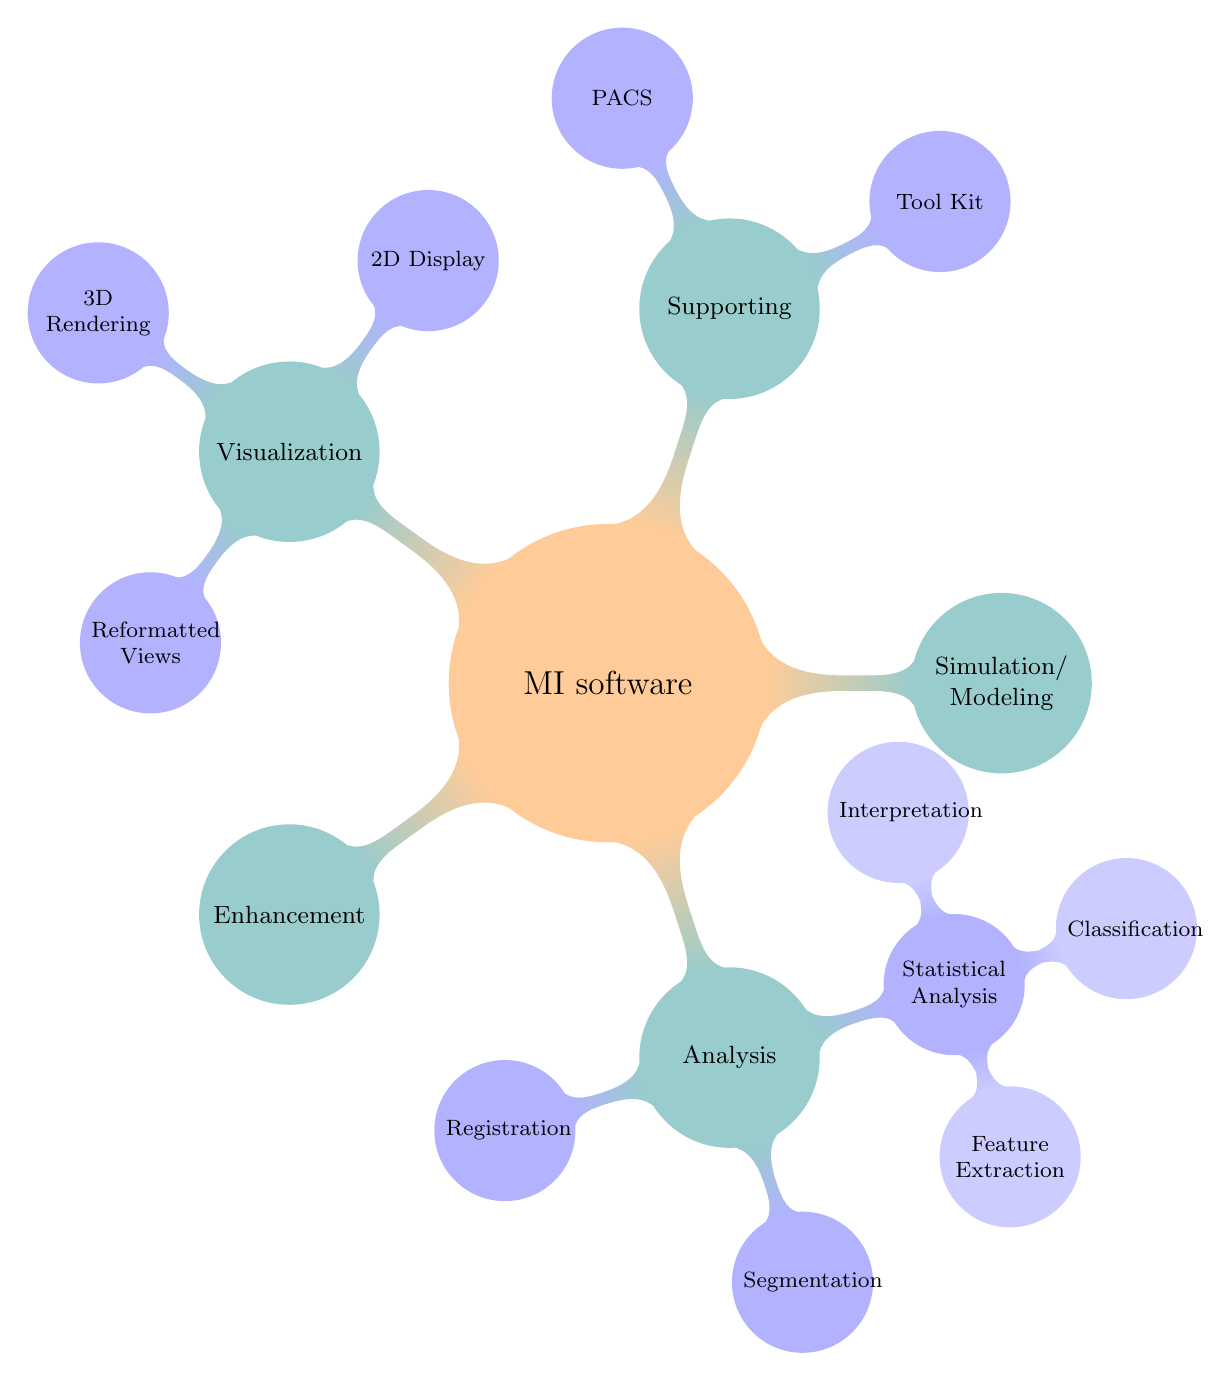
\begin{tikzpicture}[mindmap, grow cyclic, every node/.style=concept, concept
color=orange!40,
level 1/.append style={level distance=5cm,sibling angle=72},
level 2/.append style={level distance=3cm,sibling angle=90},
level 3/.style={level distance=2.3cm,sibling angle=90}]
\node{MI software}
child[concept color=teal!40] { node {Enhancement}}
child[concept color=teal!40] { node {Analysis}
    child[concept color=blue!30] { node {Registration}}
    child[concept color=blue!30,] { node {Segmentation}}
    child[concept color=blue!30] { node {Statistical Analysis}
    child[concept color=blue!20] { node {Feature Extraction}}
    child[concept color=blue!20] { node {Classification}}
    child[concept color=blue!20] { node {Interpretation}}
    }}
child[concept color=teal!40] { node {Simulation/\\Modeling}}
child[concept color=teal!40] { node {Supporting}
    child[concept color=blue!30] { node {Tool Kit}}
    child[concept color=blue!30] { node {PACS}}
}
child[concept color=teal!40] { node {Visualization}
    child[concept color=blue!30] { node {2D Display}}
    child[concept color=blue!30] { node {3D Rendering}}
    child[concept color=blue!30] { node {Reformatted Views}}
};
\end{tikzpicture}
\caption{Major functions of MI software}
\label{fig_mi_functions}
\end{figure}

To keep the data collection and analysis feasible, we limited the scope of the
software to the software packages providing the Visualization tools and
functions in this project.

[Roadmap - instead sprinkle forward references throughout the introduction?]

\section{Background} \label{ch_background}

When designing a method for evaluating the state of the practice of
domain-specific software, we included a step to select domain and software.
Knowledge of different software categories is essential for the selection. To
compare and rank the software qualities with the grading template in Appendix
\ref{ap_grading_template}, we need the definitions of qualities and the AHP.

In this section, we introduce the relevant software categories (Section
\ref{sec_software_categories}). We also cover the software quality definitions
(Section \ref{sec_software_quality}) and an overview of the AHP (Section
\ref{sec_AHP}).

\subsection{Software Categories} \label{sec_software_categories}

We target specific software categories to narrow down the scope when selecting
software packages for measuring. One way to categorize them is grouping by
functions, such as analyzing the scope for the MI software (Section
\ref{sec_scope}), which requires specific domain knowledge. In this section, we
discuss three common software categories that we can apply to all SC domains:
Open source software (OSS), freeware, and commercial software.

\subsubsection{Open Source Software} \label{sec_open_source_software}

For OSS, the source code is openly accessible. Users have the right to study,
change and distribute it under a license granted by the copyright holder. For
many OSS projects, the development process relies on the collaboration of
different contributors worldwide \citep{Corbly2014}. Accessible source code
usually exposes more ``secrets'' of a software project, such as the underlying
logic of software functions, how developers achieve their works, and the flaws
and potential risks in the final product. Thus, it brings much more convenience
to researchers analyzing the qualities of the project.

\subsubsection{Freeware} \label{sec_freeware}

Freeware is software that can be used free of charge. Unlike with OSS, the
authors of freeware do not allow users to access or modify the source code of
the software \citep{LINFO2006}. The term \textit{freeware} should not be confused
with \textit{free software}, which is similar to OSS. To the end-users, the
differences between freeware and OSS often do not bother them. The fact that
these products are free of charge is likely to make them popular with many
users. However, software developers, end-users who wish to modify the source
code, and researchers looking for insight into software development process will
find the inaccessible source code a problem. 

\subsubsection{Commercial Software}

``Commercial software is software developed by a business as part of its
business'' \citep{GNU2019}. Typically speaking, the users are required to pay to
access all of the features of commercial software, excluding access to the
source code. However, some commercial software is also free of charge
\citep{GNU2019}. Based on our experience, most commercial software products are
not OSS.

For some specific software, the backgrounds of commercial software developers
often differ from the ones of non-commercial OSS. In such a case, the former is
usually the product of software engineers, and the latter is likely to have
developers who work in the domain and are also end-users of the products. One
example of such software is SC software, since the developers need to utilize
their domain-specific during the development process \citep{Wilson2014}.

\subsection{Software Quality Definitions} \label{sec_software_quality}

This section lists the definitions of 10 software qualities, which are from
Smith et al. \citep{SmithEtAl2020}. We aim to measure each of them for selected
SC software packages. The order of the first nine qualities follows our grading
template in Appendix \ref{ap_grading_template}. We do not measure
\textit{reproducibility} with the grading template, but discuss it with the
developers by interviews.

\begin{itemize}
	\item \textbf{Installability} The effort required for the installation,
	uninstallation, or reinstallation of a software or product in a specified
	environment \citep{ISO/IEC25010} \citep{lenhard2013measuring}.

	\item \textbf{Correctness \& Verifiability} A program is correct if it
	behaves according to its stated specifications. Verifiability is the extent
	to which a set of tests can be written and executed, to demonstrate that the
	delivered system meets the specification \citep{GhezziEtAl2003}.

	\item \textbf{Reliability} The probability of failure-free operation of a
	computer program in a specified environment for a specified time, i.e., the
	average time interval between two failures also known as the mean time to
	failure (MTTF) \citep{musa1987software} \citep{GhezziEtAl2003}.

	\item \textbf{Robustness} Software possesses the characteristic of
	robustness if it behaves ``reasonably'' in two situations: i) when it
	encounters circumstances not anticipated in the requirements specification,
	and ii) when the assumptions in its requirements specification are violated
	\citep{ghezzi1991fundamentals} \citep{boehm2007software}.

	\item \textbf{Usability} ``The extent to which a product can be used by
	specified users to achieve specified goals with effectiveness, efficiency,
	and satisfaction in a specified context of use" \citep{ISO/TR16982:2002}
	\citep{ISO9241-11:2018}.

	\item \textbf{Maintainability} The effort with which a software system or
	component can be modified to i) correct faults; ii) improve performance or
	other attributes; iii) satisfy new requirements
	\citep{IEEEStdGlossarySET1990} \citep{boehm2007software}.

	\item \textbf{Reusability} ``The extent to which a software component can be
	used with or without adaptation in a problem solution other than the one for
	which it was originally developed" \citep{kalagiakos2003non}.

	\item \textbf{Understandability} ``The capability of the software product to
	enable the user to understand whether the software is suitable, and how it
	can be used for particular tasks and conditions of use" \citep{iso2001iec}.

	\item \textbf{Visibility/Transparency} The extent to which all of the steps
	of a software development process and the current status of it are conveyed
	clearly \citep{ghezzi1991fundamentals}.

	\item \textbf{Reproducibility} ``A result is said to be reproducible if
	another researcher can take the original code and input data, execute it,
	and re-obtain the same result" \citep{BenureauAndRougier2017}.
\end{itemize}

\subsection{Analytic Hierarchy Process} \label{sec_AHP}

To generate ranking scores for a set of software packages, we use AHP, which
utilizes pairwise comparisons between all of the packages. Thomas L. Saaty
developed this tool, and people widely used it to make and analyze multiple
criteria decisions \citep{VaidyaEtAl2006}. AHP organizes multiple criteria
factors in a hierarchical structure and uses pairwise comparisons between
alternatives to calculate relative ratios \citep{Saaty1990}.

For a project with $ m $ criteria, we can use an $m\times m$ matrix $A$ to
record the relative importance between factors. When comparing criterion $i$ and
criterion $j$, the value of $A_{ij}$ is decided as follows, and the value of
$A_{ji}$ is $1/A_{ij}$ \citep{Saaty1990},

\begin{itemize}
	\item $A_{ij} = 1$ if criterion $i$ and criterion $j$ are equally important;
	\item $A_{ij} = 9$ if criterion $i$ is extremely more important than
	criterion $j$;
	\item $A_{ij}$ equals to an integer value between 1 and 9 according the the
	relative importance of criterion $i$ and criterion $j$.
\end{itemize}

The above process assumes that criterion $i$ is not less important than
criterion $j$, otherwise, we need to reverse $i$ and $j$ and determine $A_{ji}$
first, then $A_{ij} = 1/A_{ji}$.

The priority vector $w$ can be calculated by solving the following equation
\citep{Saaty1990}, 
\begin{equation} 
    Aw = \lambda_{max}w,
\end{equation}
where $\lambda_{max}$ is the maximal eigenvalue of $A$.

In this project, $w$ is approximated with the classic \textit{mean of normalized
values} approach \citep{AlessioEtAl2006},

\begin{equation}
w_i = \frac{1}{m}\sum_{j=1}^{m}\frac{A_{ij}}{\sum_{k=1}^{m}A_{kj}}
\end{equation}

Suppose there are $n$ alternatives, for criterion $i = 1, 2, ... , m$, we can
create an $n\times n$ matrix $B_i$ to record the relative preferences between
these choices. The way of generating $B_i$ is similar to the one for $A$.
However, unlike comparing the importance between criteria, we pairwise decide
how much we favor one alternative over the other. We use the same method to
calculate the local priority vector for each $B_i$.

In this project, the first nine software qualities mentioned in Section
\ref{sec_software_quality} are the criteria ($m = 9$), while 29 software
packages ($n = 29$) are compared for each of the $m$ criteria. The software are
evaluated with the grading template in Appendix \ref{ap_grading_template} and a
subjective score from one to ten is given for each quality for each package. For
each quality, for a pair of packages $i$ and $j$, such that $score_i >=
score_j$, the difference between two scores is $\mathit{diff_{ij}} = score_i -
score_j$. The relationship between $A_{ij} = 1$ and $\mathit{diff_{ij}}$ is as
follows:

\begin{itemize}
\item $A_{ij} = 1$ and $\mathit{diff_{ij}} = 0$ when criterion $i$ and criterion
$j$ are equally important;
\item $A_{ij}$ increases when $\mathit{diff_{ij}}$ increases;
\item $A_{ij} = 9$ and $\mathit{diff_{ij}} = 9$ when criterion $i$ is extremely
more important than criterion $j$.
\end{itemize}

Thus, we approximate the pairwise comparison result of $i$ versus $j$ by the
following equation:

\begin{equation}
A_{ij} = min(score_i - score_j + 1, 9)
\end{equation}

\section{Methodology} \label{ch_methods}

We designed a general process for evaluating the state of the practice of
domain-specific SC software, that we instantiate for a specific scientific
domain.

Our method involves four steps:
\begin{enumerate}
\item choosing a software domain (Section \ref{sec_domain_selection});
\item collecting and filtering software packages (Section
\ref{sec_software_selection});
\item grading the selected software (Section \ref{sec_grading_software});
\item interviewing development teams for further information (Section
\ref{sec_interview_methods}).
\end{enumerate}

\noindent Section \ref{sec_applying_method} presents an example of how we
applied the method on the MI domain.

\subsection{Domain Selection} \label{sec_domain_selection}

Our methods are generic for any SC software, but they need to be applied to a
specific domain. When choosing a candidate domain, we prefer one with a large
number of active OSS. The reason is that we aim to finalize a list of 30
software packages \citep{SmithEtAl2021} after the screening step. For example, we
remove the ones without recent updates or specific functions. Besides, we prefer
OSS projects because our grading method requires access to the code. In
addition, we prefer a domain with an active community developing and using the
software. As a result, it is easier to invite enough developers for interviews.

We prefer 30 software packages providing similar functions or falling into
different sub-groups depending on our research purpose. So the domain needs to
have enough candidates in one sub-group or enough sub-groups to cross-compare.

We also prefer domains in which our team has expertise. We invite domain experts
to join and support our projects. They help us in many aspects, such as vetting
the software list and interview questions.

\subsection{Software Product Selection} \label{sec_software_selection}

The process of selecting software packages contains two steps: i) identify
software candidates in the chosen domain, ii) filter the list according to our
needs \citep{SmithEtAl2021}.

\subsubsection{Identify Software Candidates} \label{sec_identify_software_candidates}

We start with finding candidate software in publications of the domain. Then, we
search various websites, such as \hyperlink{https://github.com/}{GitHub},
\hyperlink{https://swmath.org/}{swMATH} and the Google search results for
software recommendation articles. We should also include the ones suggested by
the domain experts \citep{SmithEtAl2021}.

\subsubsection{Filter the Software List} \label{sec_filter_software_list}

The goal is to build a software list with a length of about 30
\citep{SmithEtAl2021}.

The only ``mandatory'' requirement is that the software must be OSS, as defined
in Section \ref{sec_open_source_software}. We need this because evaluating some
software qualities requires the source code.

The other filters are optional, and we consider them according to the number of
software candidates and the objectives of the research project. We apply them in
the following priority order:

\begin{enumerate}
\item The functions and purpose of the software. An SC domain often contains
software with various functions and purposes. For example, some MI software
packages are Tool Kit for developers to use, and some others offer Visualization
function to end-users. We have two options:
\begin{itemize}
\item selecting a set of software with the same major function. In this case, we
can use the identical process to assess all packages, e.g., same input to
measure \textit{Robustness}. Also, when we give impression scores to qualities
such as \textit{Installability} and \textit{Usability}, the results are more
comparable. Thus, it is more feasible to collect the results and rank the
software.
\item selecting software from a set of different sub-groups. For example, we can
choose 10 MI software from each of the three sub-groups: Visualization, Tool
Kit, and PACS. The downside: we may need different processes to measure each
sub-group; it may be less accurate to mix all three sub-groups and rank them
together. The benefit: we can cross-compare the development processes between
the sub-groups.
\end{itemize}

\item The version control tool. The empirical measurement tools listed in
Section \ref{sec_empirical_measurements} only work on projects using
\hyperlink{https://git-scm.com/}{Git}, so we prefer software with Git. Some
manual steps in empirical measurement depend on a few metrics of GitHub, which
makes projects held on GitHub more favored \citep{SmithEtAl2021}.

\item The age of the software. Some of the OSS projects may experience a lack of
recent maintenance. So we eliminate packages without recent updates, unless they
are still popular and highly recommended by the domain users
\citep{SmithEtAl2021}. We consider a software project as ``alive" if it has any
update within the last 18 months; otherwise, we mark it as ``dead".
\end{enumerate}

The order of filters 2 and 3 is flexible. We adjust it according to the number
of software packages affected by the filters, and the number of ones remaining
on the list.

\subsubsection{Vet the Software List} \label{sec_vet_software_list}

Before showing our filtered list to the domain experts, we ask them to list
their top 10 software in the domain. Then, we cross-compare the two lists and
discuss the commonality and variability.  In addition, we ask them to vet our
filtered list. They provide views on whether the list is reasonable. We also use
their opinions for a filtering process. For example, if a software package is
not OSS and has had no updates for a long time, but the domain experts identify
it as a valuable product, we still consider it in our final list.

\subsection{Grading Software} \label{sec_grading_software}

We grade the selected software using a template (Section
\ref{sec_grading_template}) and a specific empirical method (Section
\ref{sec_empirical_measurements}). Some technical details for the measurements
are in Section \ref{sec_technical_details}.

\subsubsection{Grading Template} \label{sec_grading_template}

The full grading template can be found in Appendix \ref{ap_grading_template}.
The template contains 103 questions that we use for grading software products.
Figure \ref{fg_grading_template_example} shows an example of this grading
template.

\begin{figure}[ht]
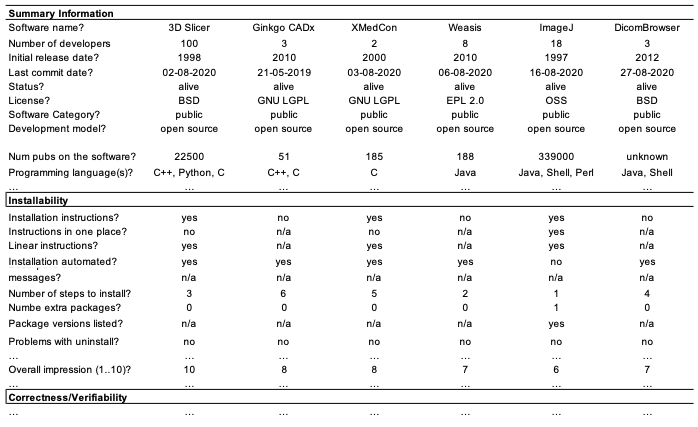
\includegraphics[scale=0.42]{figures/template.png}
\caption{Grading template example}
\label{fg_grading_template_example}
\end{figure}

We use the first section of the template to collect general information, such as
the name, purpose, platform, programming language, publications about the
software, the first release and the most recent change date, website, source
code repository of the product, etc. Information in this section helps us
understand the projects better and may be helpful for further analysis, but it
does not directly affect the grading scores.

We designed the following nine sections in the template for the nine software
qualities mentioned in Section~\ref{sec_software_quality}. For each quality, we
ask several questions and the typical answers are among the collection of
``yes'', ``no'', ``n/a'', ``unclear'', a number, a string, a date, a set of
strings, etc. Each quality needs an overall score between 1 and 10 based on all
the previous questions. For some qualities, we perform surface measurements,
which allow us to measure all packages with reasonable efforts. The surface
measurements reveal some traits of a underlying quality, but may not fully
represent it.

\begin{itemize}

\item \textbf{Installability} We check the existence and quality of installation
instructions. The user experience is also an important factor, such as the ease
to follow the instructions, number of steps, automation tools, and the
prerequisite steps for the installation. If any problem interrupts the process
of installation or uninstallation, we give a lower score to this quality. We
also record the Operating System (OS) for the installation test and whether we
can verify the installation.

\item \textbf{Correctness \& Verifiability} For \textit{correctness}, we check
the projects to identify the techniques to ensure this quality, such as literate
programming, automated testing, symbolic execution, model checking, unit tests,
etc. We also examine whether the projects use continuous integration and
continuous delivery (CI/CD). For \textit{verifiability}, we go through the
documents of the projects to check the requirements specifications, theory
manuals, and getting started tutorials. If a getting started tutorial exists and
provides expected results, we follow it and check if the outputs match.

\item \textbf{Surface Reliability} We check whether the software breaks during
the installation and the operations following a getting started tutorials,
whether there are descriptive error messages, and if we can recover the process
after an error. We use the software to load damaged images during the assessment
to \textit{surface robustness}, and lower its score for \textit{surface
reliability} if a software product ``break" in this process.

\item \textbf{Surface Robustness} We check how the software handles
unexpected/unanticipated input. For example, we prepare broken image files for
MI software packages with the function to load image files. We use a text file
(.txt) with a modified extension name (.dcm) as an unexpected/unanticipated
input. We load a few correct input files to ensure the function is working
correctly before testing with the unexpected/unanticipated ones.

\item \textbf{Surface Usability} We examine the documentation of the projects,
and we consider software with a getting started tutorial and a user manual
easier to use. Meanwhile, we check if users have any channels to get support. We
also record our impressions and user experiences when testing the software.
Easy-to-use graphical user interfaces give us a better experience, which leads
to better scores.

\item \textbf{Maintainability} We search the projects' documents and identify
the process of contributing and reviewing code. We believe that the artifacts of
a project - including source code, documents, building scripts, etc. - can
significantly affect its  \textit{maintainability}. Thus we check each project
for its artifacts, such as API documentation, bug tracker, release notes, test
cases, build files, version control, etc. We also check the tools supporting
issue tracking and version control, the percentages of closed issues, and the
proportion of comment lines in code.

\item \textbf{Reusability} We count the total number of code files for each
project. Projects with a large number of components provide more choices to
reuse. Furthermore, well-modularized code, which tends to have smaller parts in
separated files, is typically easier to reuse. Thus, we consider the projects
with more code files and less code lines per file to be more reusable. We use a
command-line tool \textit{scc} to count the number of  text-based files and LOC
for all projects. We also decide that the projects with API documentation can
deliver better \textit{Reusability}.

\item \textbf{Surface Understandability} We randomly examine 10 code files. We
check the code’s style within each file, such as whether the identifiers,
parameters, indentation, and formatting are consistent, whether the constants
(other than 0 and 1) are hardcoded, and whether the developers modularized the
code. We also check the descriptive information for the code, such as documents
mentioning the coding standard, the comments in the code, and the descriptions
or links for algorithms in the code. 

\item \textbf{Visibility/Transparency} To measure this quality, we check the
existing documents to find out whether the software development process and
current status of a project are visible and transparent. We examine the
development process, current status, development environment, and release notes
for each project. If any information is missing or poorly conveyed, the
\textit{visibility/transparency} will be lower.
\end{itemize}

For some qualities, the empirical measurements also affect the score. We use
tools to extract information from the source code repositories. For projects
held on GitHub, we manually collect additional metrics, such as the stars of the
GitHub repository, and the numbers of open and closed pull requests. Section
\ref{sec_empirical_measurements} presents more details about the empirical
measurements.

\subsubsection{Empirical Measurements} \label{sec_empirical_measurements}

We use two command-line tools for the empirical measurements. One is
\textit{GitStats} that generates statistics for git repositories and displays
outputs in the form of web pages \citep{Gieniusz2019}; the other one is Sloc Cloc
and Code (as known as \textit{scc}) \citep{Boyter2021}, aiming to count the lines
of code, comments, etc.

Both tools measure the number of text-based files in a git repository and lines
of text in these files. Based on our experience, most text-based files in a
repository contain programming source code, and developers use them to compile
and build software products. A minority of these files are instructions and
other documents. So we roughly regard the lines of text in text-based files as
lines of programming code. The two tools usually generate similar but not
identical results. From our understanding, this minor difference is due to the
different techniques to detect if a file is text-based or binary.

Additionally, we manually collect information for projects held on GitHub, such
as the numbers of stars, forks, people watching this repository, open pull
requests, closed pull requests, and the number of months a repository has been
on GitHub. A git repository can have a creation date much earlier than the first
day on GitHub. For example, the developers created the git repository of
\textit{3D Slicer} in 2002, but did not upload a copy of it to GitHub until
2020. We get the creation date of the GitHub copy by using API
\textit{https://api.github.com/repos/{:owner}/{:repository}} (e.g.,
\hyperlink{https://api.github.com/repos/slicer/slicer}{https://api.github.com/repos/slicer/slicer}).
In the response, the value of ``created\_at" is what we want. The number of
months a repository has been on GitHub helps us understand the average change of
metrics over time, e.g., the average new stars per month. 

These empirical measurements help us from two aspects. Firstly, they help us
with getting a project overview faster and more accurately. For example, the
number of commits over the last 12 months shows how active this project has
been, and the number of stars and forks may reveal its popularity. Secondly, the
results may affect our decisions regarding the grading scores for some software
qualities. For example, if the percentage of comment lines is low, we
double-check the \textit{understandability} of the code; if the ratio of open
versus closed pull requests is high, we pay more attention to the
\textit{maintainability}.

\subsubsection{Technical Details} \label{sec_technical_details}

To test the software on a ``clean'' system, we create a new virtual machine (VM)
for each software and only install the necessary dependencies before measuring.
We make all 30 VMs on the same computer, one at a time, and destroy them after
measuring.

We spend about two hours grading each package, unless we find technical issues
and need more time to resolve them. In most of the situation, we finish all the
measurements for one software on the same day.

\subsection{Interview Methods} \label{sec_interview_methods}

This section introduces our interview questions (Section
\ref{sec_interview_questions}), method of selecting interviewees (Section
\ref{sec_interviewee_selection}), and interview process (Section
\ref{sec_interview_process}).

\subsubsection{Interview Questions} \label{sec_interview_questions}

We designed a list of 20 questions to guide our interviews, which can be found
in Section \ref{ch_interview} and Appendix \ref{ap_interview}.

Some questions are about the background of the software, the development teams,
the interviewees, and how they organize the projects. We also ask about their
understandings of the users. Some questions focus on the current and past
difficulties, and the solutions the team has found or will try. We also discuss
the importance and current situations of documentation. A few questions are
about specific software qualities, such as \textit{maintainability},
\textit{understandability}, \textit{usability}, and \textit{reproducibility}.

The interviews are semi-structured based on the question list; we ask follow-up
questions when necessary. Based on our experience, the interviewees usually
bring up some exciting ideas that we did not expect, and it is worth expanding
on these topics.

\subsubsection{Interviewee Selection} \label{sec_interviewee_selection}

For a software list with a length of roughly 30, we aim to interview about ten
development teams. Interviewing multiple individuals from each team gives us
more comprehensive information, but a single engineer well-knowing the project
is also sufficient.

Ideally, we select projects after the grading measurements and prefer the ones
with higher overall scores. However, if we do not find enough participants, we
reach all teams on the list. As mentioned in Section
\ref{sec_apply_to_mi_interviews}, when we applied this process to the MI domain,
we eventually contacted all teams.

We try to find the contacts of the teams on the projects' websites, such as the
official web pages, repositories, publications, and bio pages of the teams'
institutions. Then, we send at most two emails to one contact asking for its
participation before receiving any replies. We operate the invitation according
to our ethics approval, such as the one in Appendix \ref{ap_ethics}. For
example, we ask for participants' consent before interviewing them, recording
the conversation, or including it in our report.

\subsubsection{Interview Process} \label{sec_interview_process}

Before contacting any interviewee candidate, we need to receive ethics clearance
from the McMaster University Research Ethics Board. Since the members of the
development teams are usually around the world, we organize these interviews as
virtual meetings online with \hyperlink{https://zoom.us/}{Zoom}. After receiving
consent from the interviewees, we also record and transcribe our discussions.

\subsection{Applying the Method to MI} \label{sec_applying_method}

This section shows an overview of applying our method to the MI domain.

\subsubsection{Domain Selection}

Based on the principles in Section \ref{sec_domain_selection}, we selected the
MI domain and the sub-group of software with the Visualization function shown in
Figure \ref{fig_mi_functions}. We also included Dr. Michael Noseworthy, a
professor of Electrical and Computer Engineering at McMaster University,
Co-Director of the McMaster School of Biomedical Engineering, and Director of
Medical Imaging Physics and Engineering at St. Joseph’s Healthcare, and some of
his students as the MI domain experts in our team.

\subsubsection{Software Product Selection} \label{sec_mi_software_selection}

By using the method in Section \ref{sec_identify_software_candidates}, we
identified 48 MI software projects as the candidates from publications
\citep{Bjorn2017} \citep{Bruhschwein2019} \citep{Haak2015}, online articles related
to the domain \citep{Emms2019} \citep{Hasan2020} \citep{Mu2019}, forum discussions
related to the domain \citep{Samala2014}, etc. Appendix
\ref{ap_list_before_filtering} shows all 48 software packages.

Guided by the method in Section \ref{sec_filter_software_list}, we filtered the
list with a process as follows:

\begin{enumerate}

\item Among them, there were eight that we could not find their source code,
such as \textit{MicroDicom}, \textit{Aliza}, and \textit{jivex}. These packages
are likely to be freeware defined in Section \ref{sec_freeware} and not OSS. So
following guidelines in Section \ref{sec_filter_software_list} we removed them
from the list.

\item Next, we focused on the MI software providing Visualization functions, as
described in Section \ref{sec_scope}. Seven of the software on the list were
Tool Kits or libraries for other software to use as dependencies, but not for
end-users to view medical images, such as \textit{VTK}, \textit{ITK}, and
\textit{dcm4che}; another three were PACS. We also eliminated these from the
list.

\item Finally, we removed \textit{Open Dicom Viewer} from the list because it
had not received any updates for a long time (since 2011). After that, only
\textit{MatrixUser} and \textit{AMIDE} were considered as ``dead". However, both
of them had much more recent updates (after 2017) than \textit{Open Dicom
Viewer}.

\end{enumerate}

We still preferred projects using git and GitHub and being updated recently, but
did not apply this filter since packages were already below 30. Even without
this filter, 27 out of the 29 software packages on the filtered list used git,
and 24 chose GitHub.

Following the process in Section \ref{sec_vet_software_list}, our domain experts
provided a list of top software that contains 12 software products (Table
\ref{tab_top_software_experts}). We compared two lists and found six common
ones.

\begin{table}[ht]
\centering
\begin{tabular}{ll}
\hline
Software & On both lists \\ \hline
3D Slicer & X \\
Horos & X \\
ImageJ & X \\
Fiji & X \\
AFNI &  \\
FSL &  \\
Freesurfer &  \\
Mricron & X \\
Mango & X \\
Tarquin &  \\
Diffusion Toolkit &  \\
MRItrix &  \\ \hline
\end{tabular}
\caption{\label{tab_top_software_experts}Top software by the MI domain experts}
\end{table}

We included \textit{Mango} in the initial list, but removed it because it was
not OSS. However, we kept \textit{Papaya}, a the web version of \textit{Mango}.
Instead of \textit{MRIcron}, we chose \textit{MRIcroGL}, because
\textit{MRIcron} development had moved to \textit{MRIcroGL} \citep{Rorden2021b}.

Six software packages on the domain experts' list were not on our filtered list.
We believed their primary function was Analysis mentioned in Section
\ref{sec_scope}. Thus, we did not include them in our final list.

After vetting our filtered list, the domain experts believed it was reasonable
and did not identify any problem. Thus, as shown in Appendix
\ref{ap_list_before_filtering}, eventually, we had 29 software products on the
final list. 

\subsubsection{Grading Software}
\label{sec_applying_method_grading}
Then we followed the steps in Section \ref{sec_grading_software} to measure and grade the software. 27 out of the 29 packages are compatible with two or three different OS such as Windows, macOS, and Linux, and 5 of them are browser-based, making them platform-independent. However, in the interest of time, we only performed the measurements for each project by installing it on one of the platforms, most likely Windows.

\subsubsection{Interviews}
\label{sec_apply_to_mi_interviews}
We received ethics clearance from the McMaster University Research Ethics Board
(Appendix \ref{ap_ethics}). Going through the interview process in Section
\ref{sec_interview_methods}, we contacted all of the 29 teams. Members from
eight teams responded and agreed to participate. As a result, we interviewed
nine developers and architects from the eight teams.

\section{Measurement Results} \label{ch_results}

As discussed in Section~\ref{sec_grading_software}, we use a grading template
and a empirical method to measure the selected software. We applied this step to
the MI domain (Section~\ref{sec_applying_method_grading}). This section shows
the summary of the measurement results. The detailed data can be found in the
repository
\hyperlink{https://data.mendeley.com/datasets/k3pcdvdzj2/1}{https://data.mendeley.com/datasets/k3pcdvdzj2/1}.
This section contains part of the answers to \hyperlink{rq5}{RQ5}.

Table \ref{tab_final_list} shows the 29 software packages that we measured,
along with some summary data collected in the year 2020. As mentioned in Section
\ref{sec_grading_template}, we used \textit{scc} (Section
\ref{sec_empirical_measurements}) to count the Lines of Code (LOC), excluding
the comment and blank lines. We arrange the items in the descending order of the
LOC. We found the initial release dates (Rlsd) in their documents for most
projects and marked the two unknown dates with ``?". We used the date of the
latest change to each code repository to decide the latest update. We found out
funding information (Fnd) for only eight projects.

We counted the number of contributors (NOC). We considered anyone who made at
least one accepted commit to the source code as a contributor. Thus, the NOC is
not usually the same as the number of long-term members. Many of these projects
received change requests and code from the community, such as pull requests and
git commits on GitHub.

Table \ref{tab_final_list} also shows the supported OS for each software
package. Twenty-five of them could work on all three OSs: Windows (W), macOS
(M), and Linux (L). However, there was a significant difference in the
philosophy to achieve cross-platform compatibility. Most of them were native
software products, but five were naturally platform-independent web
applications, as shown in column ``Web".

\begin{table}[ht]
\centering
\begin{tabular}{llllllllll}
\hline
\multirow{2}{*}{Software} & \multirow{2}{*}{Rlsd} & \multirow{2}{*}{Updated} & \multirow{2}{*}{Fnd} & \multirow{2}{*}{NOC} & \multirow{2}{*}{LOC} & \multicolumn{3}{c}{OS} & \multirow{2}{*}{Web} \\ \cline{7-9}
 &  &  &  &  &  & W & M & L &  \\ \hline
ParaView \citep{Ahrens2005} & 2002 & 2020-10 & X & 100 & 886326 & X & X & X & X \\
Gwyddion \citep{Nevcas2012} & 2004 & 2020-11 &  & 38 & 643427 & X & X & X &  \\
Horos \citep{horosproject2020} & ? & 2020-04 &  & 21 & 561617 &  & X &  &  \\
OsiriX Lite \citep{PixmeoSARL2019} & 2004 & 2019-11 &  & 9 & 544304 &  & X &  &  \\
3D Slicer \citep{Kikinis2014} & 1998 & 2020-08 & X & 100 & 501451 & X & X & X &  \\
Drishti \citep{Limaye2012} & 2012 & 2020-08 &  & 1 & 268168 & X & X & X &  \\
Ginkgo CADx \citep{Wollny2020} & 2010 & 2019-05 &  & 3 & 257144 & X & X & X &  \\
GATE \citep{Jan2004} & 2011 & 2020-10 &  & 45 & 207122 &  & X & X &  \\
3DimViewer \citep{TESCAN2020} & ? & 2020-03 & X & 3 & 178065 & X & X &  &  \\
medInria \citep{Fillard2012} & 2009 & 2020-11 &  & 21 & 148924 & X & X & X &  \\
BioImage Suite Web \citep{Papademetris2005} & 2018 & 2020-10 & X & 13 & 139699 & X & X & X & X \\
Weasis \citep{Roduit2021} & 2010 & 2020-08 &  & 8 & 123272 & X & X & X &  \\
AMIDE \citep{Loening2017} & 2006 & 2017-01 &  & 4 & 102827 & X & X & X &  \\
XMedCon \citep{Nolf2003} & 2000 & 2020-08 &  & 2 & 96767 & X & X & X &  \\
ITK-SNAP \citep{Yushkevich2006} & 2006 & 2020-06 & X & 13 & 88530 & X & X & X &  \\
Papaya \citep{UTHSCSA2019} & 2012 & 2019-05 &  & 9 & 71831 & X & X & X &  \\
OHIF Viewer \citep{Ziegler2020} & 2015 & 2020-10 &  & 76 & 63951 & X & X & X & X \\
SMILI \citep{Chandra2018} & 2014 & 2020-06 &  & 9 & 62626 & X & X & X &  \\
INVESALIUS 3 \citep{Amorim2015} & 2009 & 2020-09 &  & 10 & 48605 & X & X & X &  \\
dwv \citep{Martelli2021} & 2012 & 2020-09 &  & 22 & 47815 & X & X & X & X \\
DICOM Viewer \citep{Afsar2021} & 2018 & 2020-04 & X & 5 & 30761 & X & X & X &  \\
MicroView \citep{ParallaxInnovations2020} & 2015 & 2020-08 &  & 2 & 27470 & X & X & X &  \\
MatrixUser \citep{Liu2016} & 2013 & 2018-07 &  & 1 & 23121 & X & X & X &  \\
Slice:Drop \citep{Haehn2013} & 2012 & 2020-04 &  & 3 & 19020 & X & X & X & X \\
dicompyler \citep{Panchal2010} & 2009 & 2020-01 &  & 2 & 15941 & X & X &  &  \\
Fiji \citep{Schindelin2012} & 2011 & 2020-08 & X & 55 & 10833 & X & X & X &  \\
ImageJ \citep{Rueden2017} & 1997 & 2020-08 & X & 18 & 9681 & X & X & X &  \\
MRIcroGL \citep{Rorden2021} & 2015 & 2020-08 &  & 2 & 8493 & X & X & X &  \\
DicomBrowser \citep{Archie2012} & 2012 & 2020-08 &  & 3 & 5505 & X & X & X &  \\ \hline
\end{tabular}
\caption{\label{tab_final_list}Final software list}
\end{table}

Most of the projects used more than one programming language, including a
primary language that the developers used the most. Figure \ref{fig_language}
shows the primary languages versus the number of projects using them.

% temporarily comment out

% \begin{figure}[ht]
% \centering
% \begin{tikzpicture}
% \centering
% \begin{axis}
% [
% ybar,
% height=8cm,
% width=12cm,
% ylabel={Number of projects},
% xlabel={\ Primary language},
% symbolic x coords={C++, JavaScript, Java, C, Python, Pascal, Matlab},
% xtick=data,
% nodes near coords,
% nodes near coords align={vertical},
% ]
% \addplot[black,fill=blue!55!black] coordinates {(C++,11) (JavaScript,6) (Java,4) (C,3) (Python,3) (Pascal,1) (Matlab,1) };
% \end{axis}  
% \end{tikzpicture}
% \caption{\label{fig_language}Primary languages versus number of projects using them}
% \end{figure}

We failed to install \textit{DICOM Viewer}, so we could not test its
\textit{surface reliability} and \textit{surface robustness}. We kept this
software on our list because the other seven qualities do not rely on a
successful installation. Besides, the \textit{DICOM Viewer} team built it as a
plugin software for NextCloud
(\hyperlink{https://apps.nextcloud.com/}{https://apps.nextcloud.com/}) platform,
which was a unique choice we had not seen before. We wanted to keep it to enrich
the diversity.

\subsection{Installability} \label{sec_result_installability}

Figure \ref{fg_installability_scores} lists the scores of
\textit{installability}.

\begin{figure}[ht]
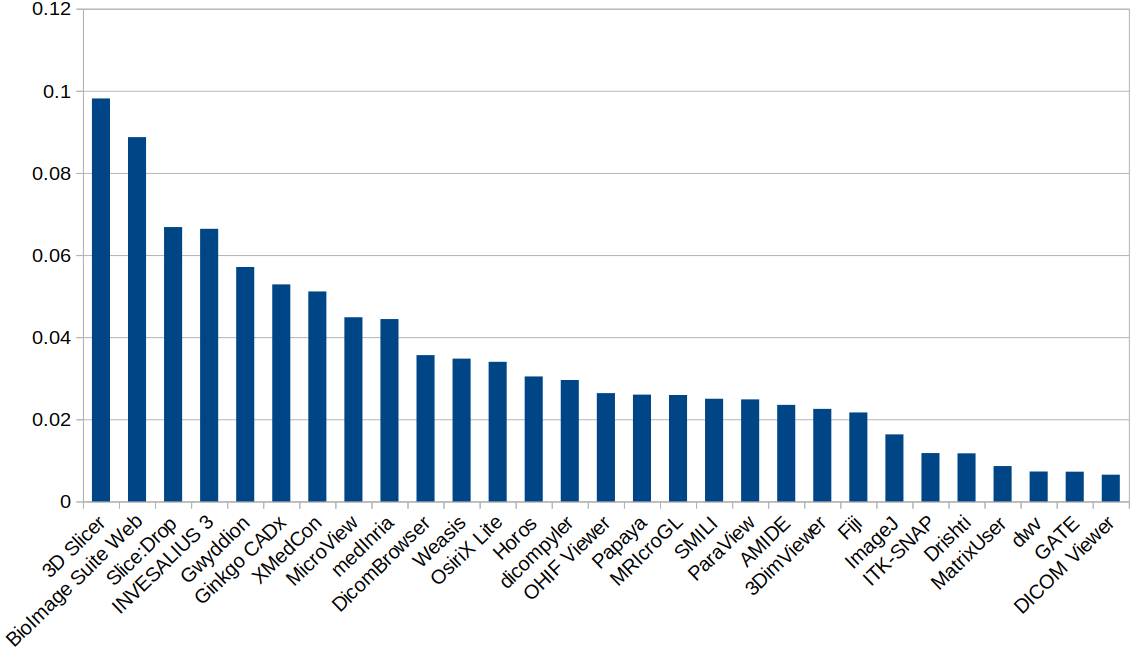
\includegraphics[scale=0.38]{figures/installability_scores.png}
\caption{AHP installability scores}
\label{fg_installability_scores}
\end{figure}

We found installation instructions for 16 projects. Among the ones without
instructions, \textit{BioImage Suite Web} and \textit{Slice:Drop} are web
applications with online versions to use, thus they do not need installation.
Installing 10 of the projects required extra dependencies. Five of them are the
web applications in Table \ref{tab_final_list}, and depended on a browser;
\textit{dwv}, \textit{OHIF Viewer}, and \textit{GATE} needed extra dependencies
to build; \textit{ImageJ} and	\textit{Fiji} needed an unzip tool;
\textit{MatrixUser} was based on Matlab; \textit{DICOM Viewer} needed to work on
a Nextcloud platform.

\textit{3D Slicer} has the highest score because it had easy to follow
installation instructions, and the installation processes were automated, fast,
and frustration-free, with all dependencies automatically added. There were also
no errors during the installation and uninstallation steps. Many other software
packages also had installation instructions and automated installers, and we had
no trouble installing them, such as \textit{INVESALIUS 3}, \textit{Gwyddion},
\textit{XMedCon}, and \textit{MicroView}. We gave them various scores based on
the understandability of the instructions, installation steps, and user
experience. Since \textit{BioImage Suite Web} and \textit{Slice:Drop} needed no
installation, we gave them higher scores. \textit{BioImage Suite Web} also
provided an option to download cache to local for offline usage, which was easy
to apply.

\textit{dwv}, \textit{GATE}, and \textit{DICOM Viewer} showed severe problems.
We could not install them. We spent a reasonable amount of time on these
problems, then considered them as major obstacles for normal users if we could
not figure out any solutions. We suspect that only a part of the users faced the
same problems, and given a lot of time, we might be able to find solutions.
However, the difficulties greatly impacted the installation experiences, and we
graded these software packages with lower scores. For example, \textit{dwv} and
\textit{GATE} had the option to build from the source code, and we failed the
building processes following the instructions. Although we could not locally
build them, we could use a deployed online version for \textit{dwv}, and a VM
version for \textit{GATE}. With those, we finished all the measurements for
them. Furthermore, \textit{DICOM Viewer} depended on the NextCloud platform, and
we could not successfully install the dependency.

\textit{MatrixUser} has a lower score because it depended on Matlab. We
considered installing Matlab takes many more steps and time, and some users may
not have a license to use Matlab.

\subsection{Correctness \& Verifiability} \label{sec_result_correctness_verifiability}

The scores of \textit{correctness \& verifiability} are shown in Figure
\ref{fg_correctness_erifiability_scores}. Generally speaking, the packages with
higher scores adopted more techniques to improve \textit{correctness}, and had
better documents for us to verify it.

\begin{figure}[ht]
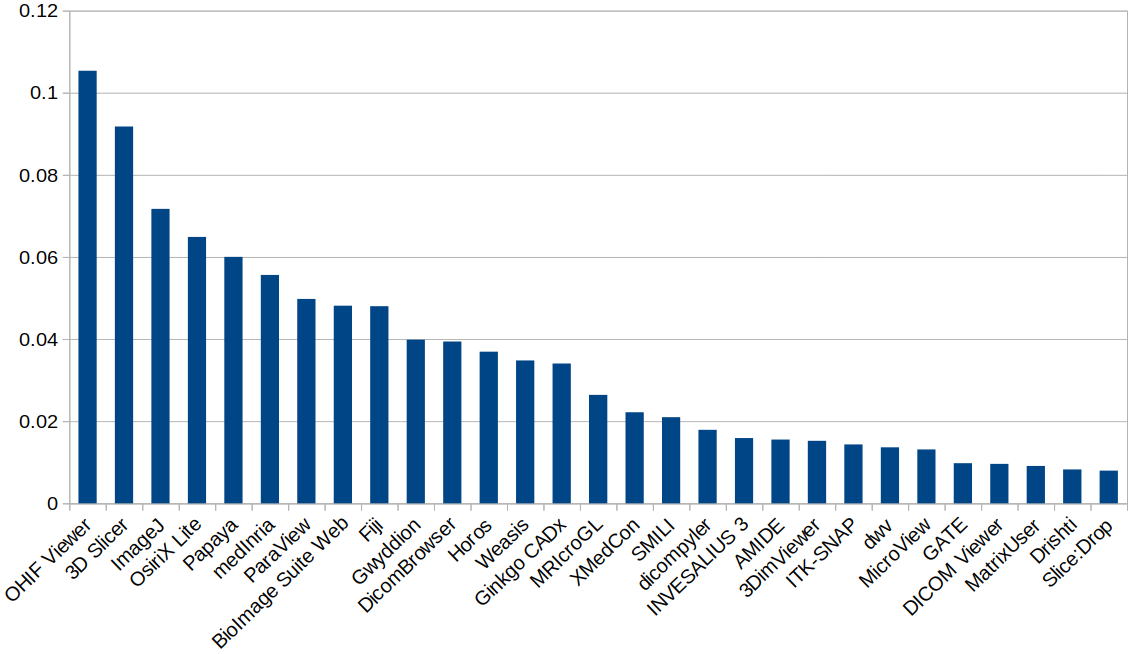
\includegraphics[scale=0.38]{figures/correctness_verifiability_scores.png}
\caption{AHP correctness \& verifiability scores}
\label{fg_correctness_erifiability_scores}
\end{figure}

After examining the source code, we could not find any evidence of unit testing
in more than half of the projects. Unit testing benefits most parts of the
software's life cycle, such as designing, coding, debugging, and optimization
\citep{Hamill2004}. It can reveal the bugs at an earlier stage of the development
process, and the absence of unit testing may cause problems for
\textit{correctness \& verifiability}.

We could not find requirements specifications for most projects. The only
document we found is a road map of \textit{3D Slicer}, which contained design
requirements for the upcoming changes. However, it did not record the conditions
for previous versions. We also could not identify the theory manuals for all of
the projects. Even for some projects with well-organized documents, requirements
specifications and theory manuals were still missing.

We identified five projects using CI/CD tools, which are \textit{3D Slicer},
\textit{ImageJ}, \textit{Fiji}, \textit{dwv}, and \textit{OHIF Viewer}.

In this section, the information about CI/CD tools is part of the answers to
\hyperlink{rq2}{RQ2}, and the information about software testing and
documentation is part of the answers to \hyperlink{rq3}{RQ3}.

\subsection{Surface Reliability} \label{sec_result_reliability}

As described in Section \ref{sec_result_installability}, we could not build
\textit{dwv} and \textit{GATE}. However, since there was an online or VM version
of them, successful deployment is possible. So the failure of installation did
not affect their scores in \textit{surface reliability}. Figure
\ref{fg_reliability_scores} shows the AHP results.

\begin{figure}[ht]
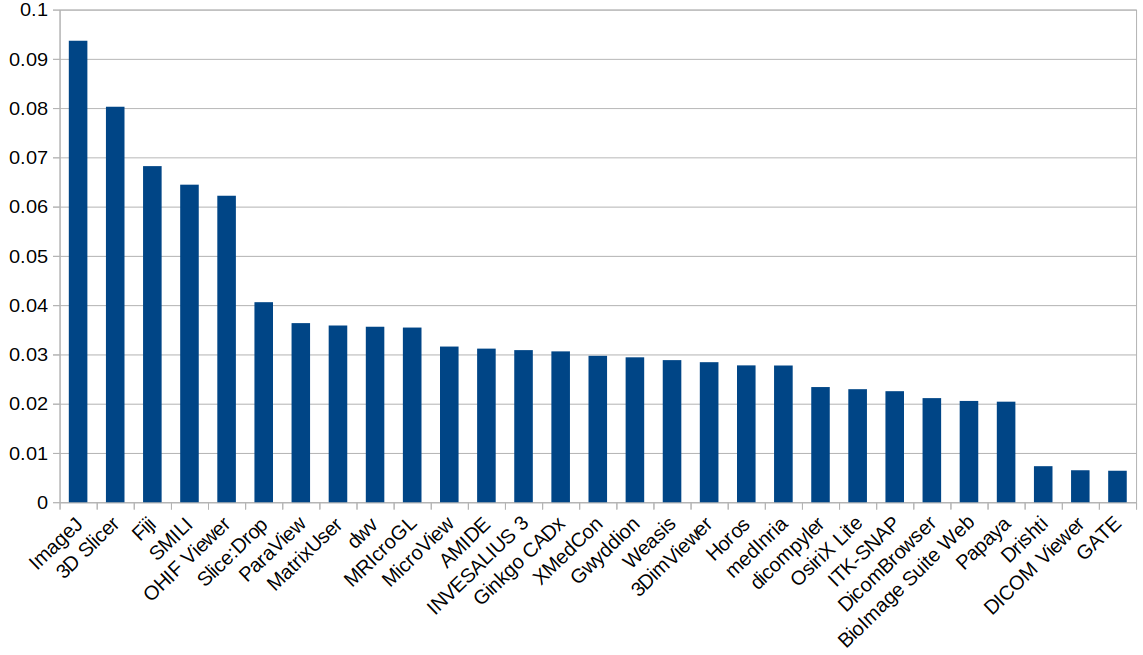
\includegraphics[scale=0.38]{figures/reliability_scores.png}
\caption{AHP surface reliability scores}
\label{fg_reliability_scores}
\end{figure}

As shown in Section \ref{sec_result_installability}, most of the software
products did not ``break" during installation or did not need installation;
\textit{dwv} and \textit{GATE} broke in the building stage, and the processes
were not recoverable; we could not install the dependency for \textit{DICOM
Viewer}.

Of the seven software packages with a getting started tutorial and operation
steps in the tutorial, most showed no error when we followed the steps. However,
\textit{GATE} could not open macro files and became unresponsive several times,
without any descriptive error message. When assessing \textit{surface
robustness} (Section \ref{sec_result_robustness}), we found out that
\textit{Drishti} crashed during loading damaged image files and did not show any
descriptive error message. On the other hand, we did not see any problems with
the online version of \textit{dwv}.

\subsection{Surface Robustness} \label{sec_result_robustness}

Figure \ref{fg_robustness_scores} presents the scores for \textit{surface
robustness}.

\begin{figure}[ht]
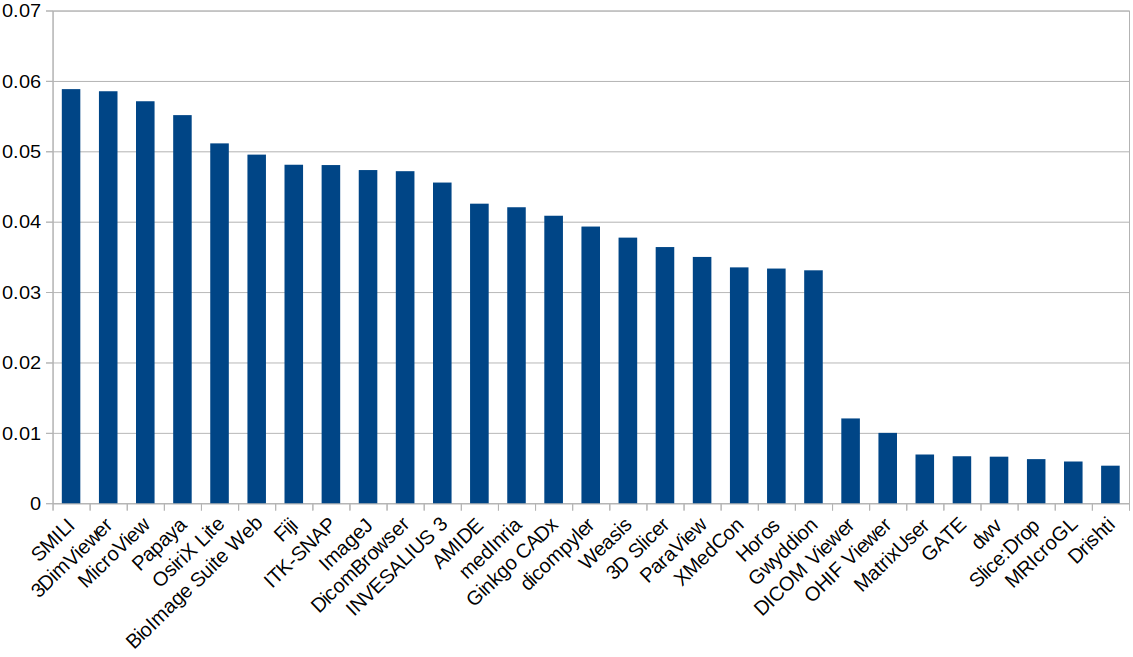
\includegraphics[scale=0.38]{figures/robustness_scores.png}
\caption{AHP surface robustness scores}
\label{fg_robustness_scores}
\end{figure}

The packages with higher scores elegantly handled the unexpected/unanticipated
inputs, typically showing a clear error message. We might underestimate the
score of \textit{OHIF Viewer} since we needed further customization to load
data, and the test was not complete.

Digital Imaging and Communications in Medicine (DICOM) is a widely used MI
standard, and ``it defines the formats for medical images that can be exchanged
with the data and quality necessary for clinical use" \citep{MITA2021}. According
to their documentation, all 29 software packages should support the DICOM
standard. We prepared two types of image files: the ones in correct formats and
the broken ones. We used two MI sample files in the DICOM format as the image
files with valid formats; we created a standard text file, changed its extension
name from ``.txt" to ``.dcm", and used it as the unexpected/unanticipated input.

Being tested with the input files with correct formats, all software packages
except \textit{GATE} loaded the images correctly. \textit{GATE} failed this test
for unknown reasons.

With the unexpected/unanticipated input, \textit{MatrixUser}, \textit{dwv}, and
\textit{Slice:Drop} ignored the incorrect format of the file and loaded it
regardless. They did not show any error message and displayed a blank image.
\textit{MRIcroGL} behaved similarly except that it showed a meaningless image
with noise pixels. \textit{Drishti} successfully detected the broken format of
the file, but the software crashed as a result. We recorded \textit{Drishti}'s
issue to the measurement of its \textit{reliability} in Section
\ref{sec_result_installability}.

\subsection{Surface Usability} \label{sec_result_usability}

Figure \ref{fg_usability_scores} lists the AHP scores for \textit{surface
usability}.

\begin{figure}[ht]
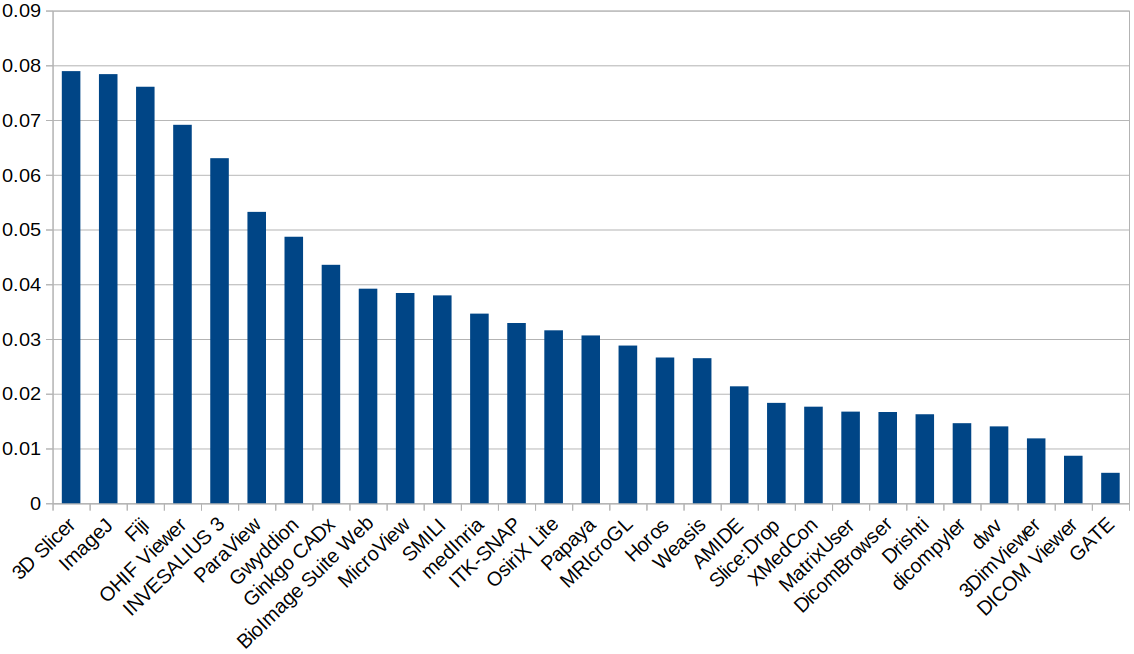
\includegraphics[scale=0.38]{figures/usability_scores.png}
\caption{AHP surface usability scores}
\label{fg_usability_scores}
\end{figure}

We found a getting started tutorial for only 11 projects but a user manual for
22 projects. \textit{MRIcroGL} was the only one with documentation for the
expected user characteristics.

The software with higher scores usually provided both comprehensive document
guidance and a good user experience. \textit{INVESALIUS 3} set an excellent
example of a detailed and precise user manual. \textit{GATE} also provided a
large number of documents, but we think that they conveyed the ideas poorly, as
we had trouble understanding and using them.
 
Table \ref{tab_user_support_model} shows the user support models by the number
of projects using them. This table contains part of the answers to
\hyperlink{rq2}{RQ2}. Maybe not every team intended to use GitHub issues to
answer users' questions, but many users use them to seek help.

\begin{table}[ht]
\centering
\begin{tabular}{ll}
\hline
\multicolumn{1}{c}{User support model} & Number of projects \\ \hline
GitHub issue & 24 \\
Frequently Asked Questions (FAQ) & 12 \\
Forum & 10 \\
E-mail address & 9 \\
GitLab issue, SourceForge discussions & 2 \\
Troubleshooting & 2 \\
Contact form & 1 \\ \hline
\end{tabular}
\caption{\label{tab_user_support_model}User support models by number of projects}
\end{table}

\subsection{Maintainability} \label{sec_score_maintainability}

Figure \ref{fg_maintainability_scores} shows the AHP results for
\textit{maintainability}. 

\begin{figure}[ht]
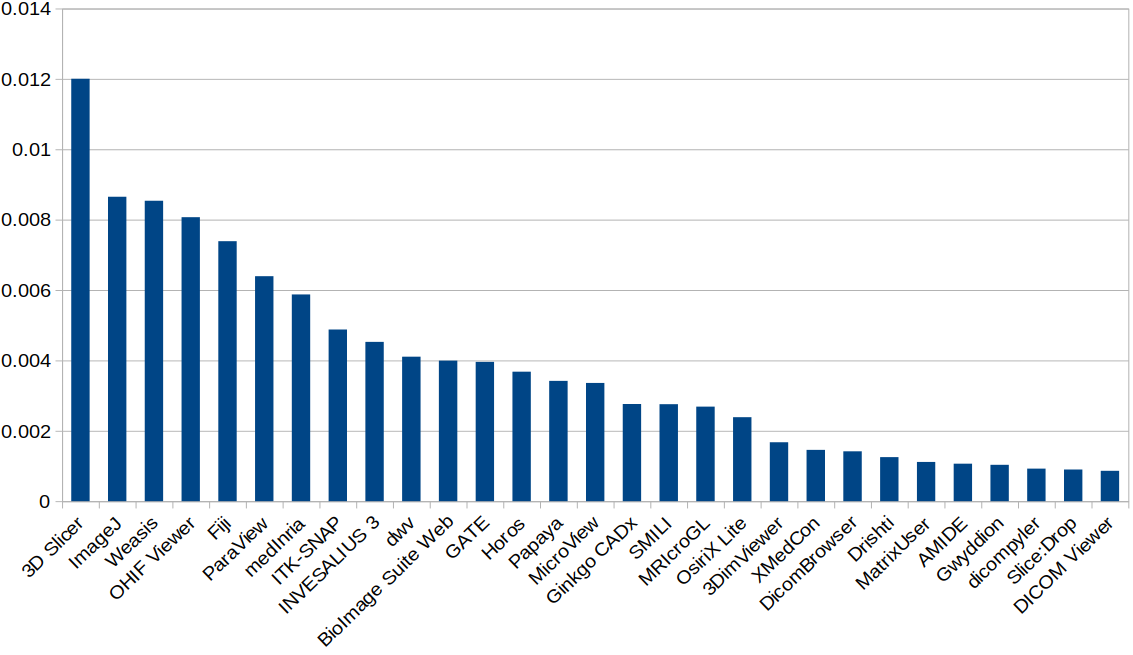
\includegraphics[scale=0.38]{figures/maintainability_scores.png}
\caption{AHP maintainability scores}
\label{fg_maintainability_scores}
\end{figure}

We marked \textit{3D Slicer} with a much higher score than others because it did
very well at closing the identified issues, and more importantly, we found it to
have the most comprehensive artifacts. For example, as far as we could find out,
only a few of the 29 projects had a project plan, developer's manual, or API
documentation, and only \textit{3D Slicer}, \textit{ImageJ}, \textit{Fiji}
included all three documents. Meanwhile, \textit{3D Slicer} has a much higher
percentage of closed issues (91.65\%) than \textit{ImageJ} (52.49\%) and
\textit{Fiji} (63.79\%). Table \ref{tab_maintainability_docs} shows which
projects had these documents, in the descending order of their
\textit{maintainability} scores. This table contains part of the answers to
\hyperlink{rq1}{RQ1} and \hyperlink{rq3}{RQ3}.

\begin{table}[ht]
\centering
\begin{tabular}{llll}
\hline
\multicolumn{1}{c}{Software} & Proj plan & Dev manual & API doc \\ \hline
3D Slicer & X & X & X \\
ImageJ & X & X & X \\
Weasis &  & X &  \\
OHIF Viewer &  & X & X \\
Fiji & X & X & X \\
ParaView & X &  &  \\
SMILI &  &  & X \\
medInria &  & X &  \\
INVESALIUS 3 & X &  &  \\
dwv &  &  & X \\
BioImage Suite Web &  & X &  \\
Gwyddion &  & X & X \\ \hline
\end{tabular}
\caption{\label{tab_maintainability_docs}Software with the maintainability documents}
\end{table}

27 of the 29 projects used git as the version control tool; \textit{AMIDE} used
Mercurial; \textit{Gwyddion} used Subversion. 24 projects used GitHub for their
repositories; \textit{XMedCon}, \textit{AMIDE}, and \textit{Gwyddion} used
SourceForge; \textit{DicomBrowser} and \textit{3DimViewer} used BitBucket. The
information about version control tools is part of the answers to
\hyperlink{rq2}{RQ2}.

\subsection{Reusability} \label{sec_result_reusability}

Figure 4.7 shows the AHP results for \textit{reusability}.

\begin{figure}[ht]
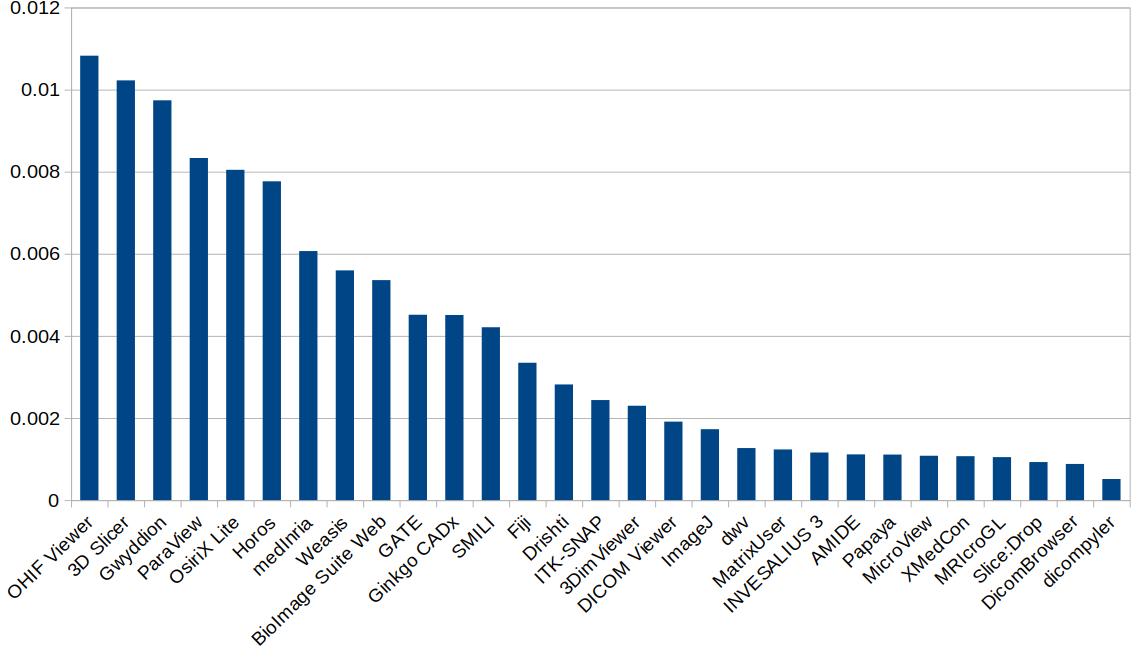
\includegraphics[scale=0.38]{figures/reusability_scores.png}
\caption{AHP reusability scores}
\label{fg_reusability_scores}
\end{figure}

As described in Section \ref{sec_grading_template}, we gave higher scores to the
projects with an API document. As shown in Table \ref{tab_maintainability_docs},
seven projects had API documents. We also considered projects with more code
files and less LOC per code file as more reusable. Table \ref{tab_loc_per_file}
shows the number of text-based files by projects, which we used to approximate
the number of code files. The table also lists the total number of lines
(including comments and blanks), LOC, and average LOC per file. We arranged the
items in the descending order of their \textit{reusability} scores. 

\begin{table}[ht]
\centering
\begin{tabular}{lllll}
\hline
\multirow{2}{*}{Software} & \multirow{2}{*}{Text files} & \multirow{2}{*}{Total lines} & \multirow{2}{*}{LOC} & \multirow{2}{*}{LOC/file} \\
 &  &  &  &  \\ \hline
OHIF Viewer & 1162 & 86306 & 63951 & 55 \\
3D Slicer & 3386 & 709143 & 501451 & 148 \\
Gwyddion & 2060 & 787966 & 643427 & 312 \\
ParaView & 5556 & 1276863 & 886326 & 160 \\
OsiriX Lite & 2270 & 873025 & 544304 & 240 \\
Horos & 2346 & 912496 & 561617 & 239 \\
medInria & 1678 & 214607 & 148924 & 89 \\
Weasis & 1027 & 156551 & 123272 & 120 \\
BioImage Suite Web & 931 & 203810 & 139699 & 150 \\
GATE & 1720 & 311703 & 207122 & 120 \\
Ginkgo CADx & 974 & 361207 & 257144 & 264 \\
SMILI & 275 & 90146 & 62626 & 228 \\
Fiji & 136 & 13764 & 10833 & 80 \\
Drishti & 757 & 345225 & 268168 & 354 \\
ITK-SNAP & 677 & 139880 & 88530 & 131 \\
3DimViewer & 730 & 240627 & 178065 & 244 \\
DICOM Viewer & 302 & 34701 & 30761 & 102 \\
ImageJ & 40 & 10740 & 9681 & 242 \\
dwv & 188 & 71099 & 47815 & 254 \\
MatrixUser & 216 & 31336 & 23121 & 107 \\
INVESALIUS 3 & 156 & 59328 & 48605 & 312 \\
AMIDE & 183 & 139658 & 102827 & 562 \\
Papaya & 110 & 95594 & 71831 & 653 \\
MicroView & 137 & 36173 & 27470 & 201 \\
XMedCon & 202 & 129991 & 96767 & 479 \\
MRIcroGL & 97 & 50445 & 8493 & 88 \\
Slice:Drop & 77 & 25720 & 19020 & 247 \\
DicomBrowser & 54 & 7375 & 5505 & 102 \\
dicompyler & 48 & 19201 & 15941 & 332 \\ \hline
\end{tabular}
\caption{\label{tab_loc_per_file}Number of files and lines}
\end{table}

\subsection{Surface Understandability} \label{sec_result_understandability}

Figure \ref{fg_surface_understandability_scores} shows the scores for
\textit{surface understandability}.

\begin{figure}[ht]
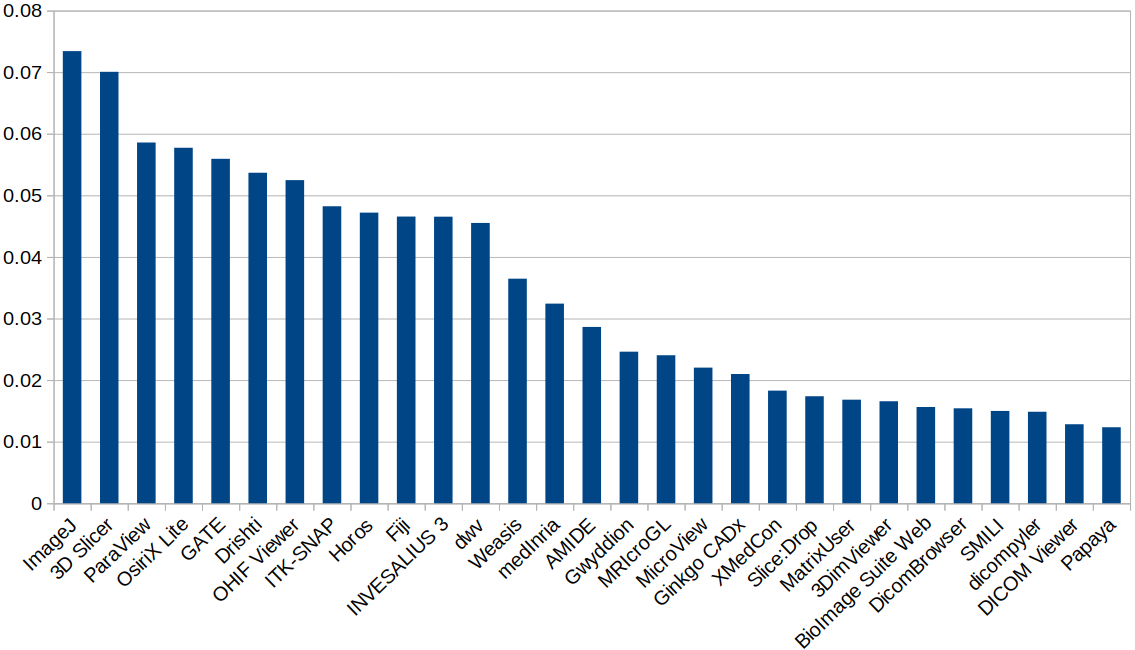
\includegraphics[scale=0.38]{figures/understandability_scores.png}
\caption{AHP surface understandability scores}
\label{fg_surface_understandability_scores}
\end{figure}

All projects had a consistent code style with parameters in the same order for
all functions; the code was modularized; the comments were clear, indicating
what is being done, not how. However, we only found explicit identification of a
coding standard for 3 out of the 29: \textit{3D Slicer}, \textit{Weasis}, and
\textit{ImageJ}. We also found hard-coded constants in \textit{medInria},
\textit{dicompyler}, \textit{MicroView}, and \textit{Papaya}. We did not find
any reference to the used algorithms in projects \textit{XMedCon},
\textit{DicomBrowser}, \textit{3DimViewer}, \textit{BioImage Suite Web},
\textit{Slice:Drop}, \textit{MatrixUser}, \textit{DICOM Viewer},
\textit{dicompyler}, and \textit{Papaya}. 

\subsection{Visibility/Transparency} \label{sec_result_visibility_transparency}

Figure \ref{fg_visibility_transparency_scores} shows the AHP scores for
\textit{visibility/transparency}. Generally speaking, the teams that actively
documented their development process and plans scored higher because they
delivered better communication to people outside the team.

\begin{figure}[ht]
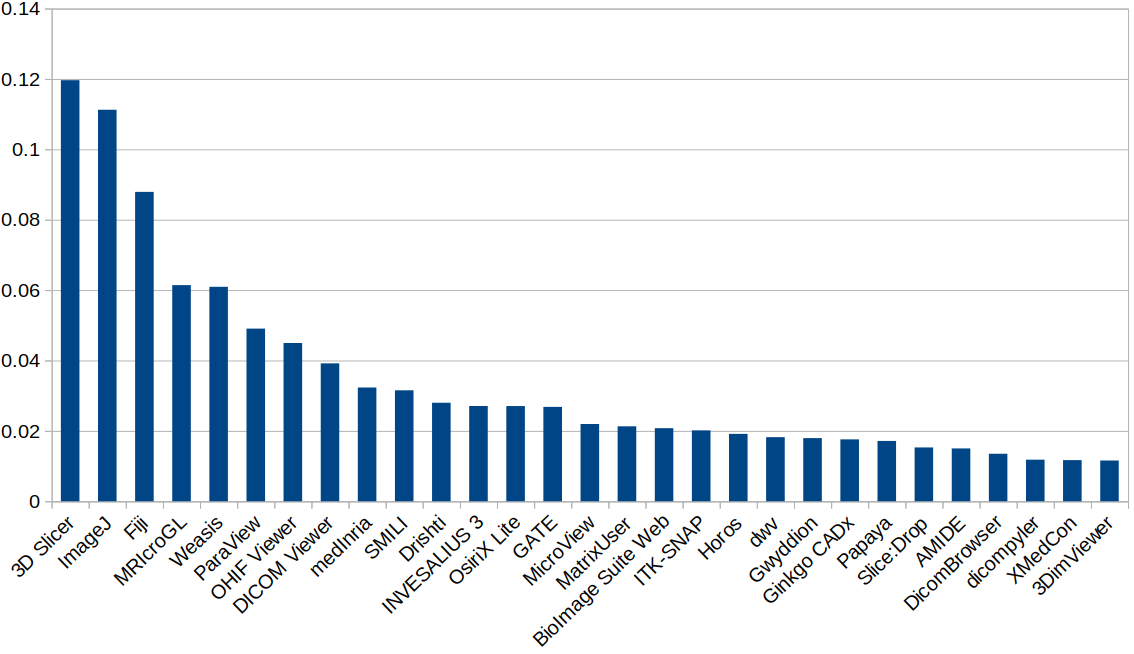
\includegraphics[scale=0.38]{figures/visibility_transparency_scores.png}
\caption{AHP visibility/transparency scores}
\label{fg_visibility_transparency_scores}
\end{figure}

Table \ref{tab_Visibility/Transparency_docs} shows the projects which had
documents for the development process, project status, development environment,
and release notes, in the descending order of their
\textit{visibility/transparency} scores. This table contains part of the answers
to \hyperlink{rq1}{RQ1} and \hyperlink{rq3}{RQ3}.

\begin{table}[ht]
\centering
\begin{tabular}{lllll}
\hline
Software & Dev process & Proj status & Dev env & Rls notes \\ \hline
3D Slicer & X & X & X & X \\
ImageJ & X & X & X & X \\
Fiji & X & X & X &  \\
MRIcroGL &  &  &  & X \\
Weasis &  &  & X & X \\
ParaView &  & X &  &  \\
OHIF Viewer &  &  & X & X \\
DICOM Viewer &  &  & X & X \\
medInria &  &  & X & X \\
SMILI &  &  &  & X \\
Drishti &  &  &  & X \\
INVESALIUS 3 &  &  &  & X \\
OsiriX Lite &  &  &  & X \\
GATE &  &  &  & X \\
MicroView &  &  &  & X \\
MatrixUser &  &  &  & X \\
BioImage Suite Web &  &  & X &  \\
ITK-SNAP &  &  &  & X \\
Horos &  &  &  & X \\
dwv &  &  &  & X \\
Gwyddion &  &  &  & X \\ \hline
\end{tabular}
\caption{\label{tab_Visibility/Transparency_docs}Software with the visibility/transparency documents}
\end{table}

\subsection{Overall Scores}

As described in Section \ref{sec_AHP}, for our AHP measurements, there are nine
criteria which are the nine software qualities and 29 software packages as the
alternatives. In the absence of requirements for an actual project, we made all
nine qualities equally important, so the score of each quality affects the
overall scores on the same scale.

Figure \ref{fg_overall_scores} shows the overall scores of all 29 software
packages in descending order. Since we produced the scores from the AHP process,
the total sum of the 29 scores is precisely 1.

\begin{figure}[ht]
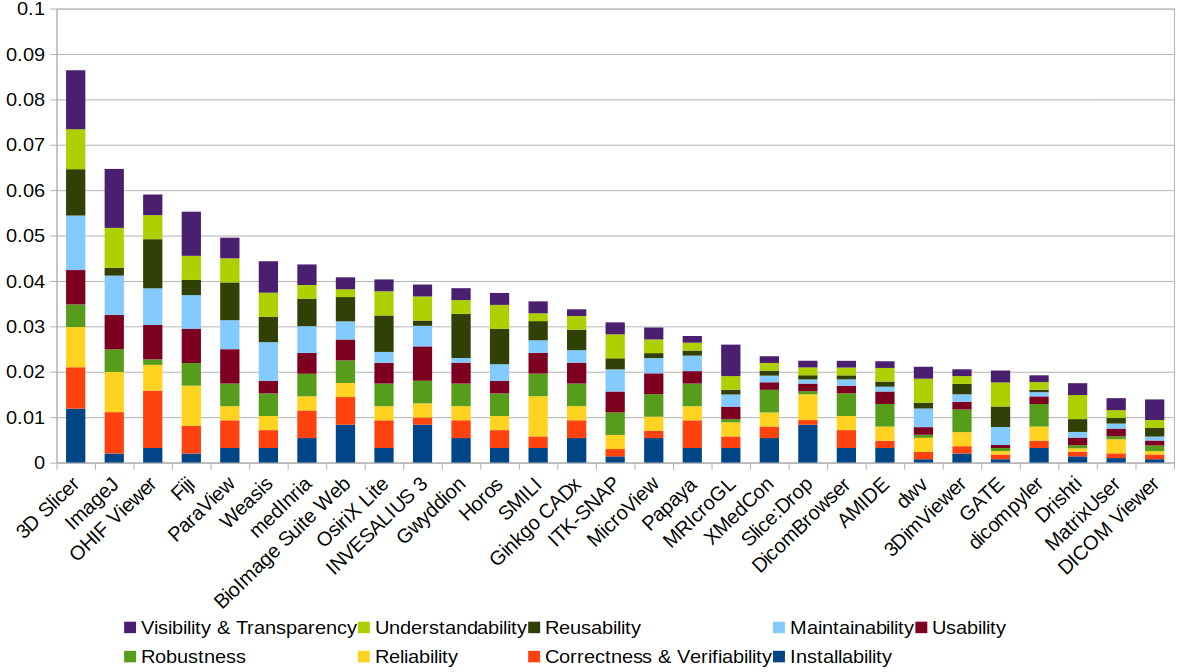
\includegraphics[scale=0.38]{figures/overall_scores.png}
\caption{Overall AHP scores for all 9 software qualities}

\label{fg_overall_scores}
\end{figure}

The top three software products \textit{3D Slicer}, \textit{ImageJ}, and
\textit{OHIF Viewer} had higher scores in most criteria. \textit{3D Slicer}
ranked in the top two software products for all qualities except \textit{surface
robustness}; \textit{ImageJ} ranked in the top three products for
\textit{correctness \& verifiability}, \textit{surface reliability},
\textit{surface usability}, \textit{maintainability}, \textit{ surface
understandability}, and \textit{visibility/transparency}; \textit{OHIF Viewer}
ranked in the top five products for \textit{correctness \& verifiability},
\textit{surface reliability}, \textit{surface usability},
\textit{maintainability}, and \textit{reusability}. We might underestimate its
scores of qualities \textit{surface reliability} and \textit{surface robustness}
for \textit{DICOM Viewer}, but equally compared it with the other software for
the rest seven qualities.

\section{Interviews with Developers} \label{ch_interview}

The measurement results in Section \ref{ch_results} are based on the information
collected by ourselves. Such information is sufficient to measure the projects
with reasonable efforts, but incomplete for us to understand the development
process more deeply. For example, we usually cannot identify the following
information in a project's documents: the pain points during the development,
the threats to certain software qualities, and the developers' strategies to
address them. We believe interviews with developers can collect the additional
information we need. As a result, our method involves interviews with developers
in a domain (Section \ref{sec_interview_methods}). We applied this step to the
MI domain (Section \ref{sec_apply_to_mi_interviews}).

In this section, we summarize some answers from the interviews. We highlight the
answers that are the most informative and interesting in this section, and
summarize the rest in Appendix \ref{ap_interview}.

As mentioned in Section \ref{sec_apply_to_mi_interviews}, we contacted all 29
teams. Some of them responded and participated in the interviews. Eventually, we
interviewed nine developers from eight of the 29 MI software projects. The eight
projects are \textit{3D Slicer}, \textit{INVESALIUS 3}, \textit{dwv},
\textit{BioImage Suite Web}, \textit{ITK-SNAP}, \textit{MRIcroGL},
\textit{Weasis}, and \textit{OHIF}. We spent about 90 minutes for each interview
and asked 20 prepared questions. We also asked following-up questions when we
thought it was worth diving deeper. One participant was too busy to have an
interview, so they wrote down their answers. The interviewees may have provided
multiple answers to each question. Thus, when counting the number of answers,
the total result is sometimes larger than nine.

\subsection{Current and Past Pain Points} \label{sec_interview_pain_points}

By asking questions \hyperlink{q9}{9}, \hyperlink{q10}{10}, and
\hyperlink{q12}{12}, we tried to identify the pain points during the development
process in the eight projects. The pain points include current and past
obstacles. We also asked the interviewees how they would solve the problems.
This section contains the answers to \hyperlink{rq4}{RQ4}. Questions 9, 10, and
12 are as follows:

\begin{description}
\item[Q9.] \hypertarget{q9}Currently, what are the most significant obstacles in
your development process?
\item[Q10.] \hypertarget{q10}How might you change your development process to
remove or reduce these obstacles?
\item[Q12.] \hypertarget{q12}In the past, is there any major obstacle to your
development process that has been solved? How did you solve it?
\end{description}

Table \ref{tab_obstacles} shows the number of times the interviewees mentioned
the current and past obstacles in their projects.

\begin{table}[ht]
\centering
\begin{tabular}{llll}
\hline
\multirow{2}{*}{Category} & \multirow{2}{*}{Obstacle} & \multicolumn{2}{c}{Num ans.} \\ \cline{3-4} 
 &  & current & past \\ \hline
\multirow{2}{*}{Resource} & Lack of fundings & 3 &  \\
 & Lack of time to devote to the project & 2 & 1 \\ \hdashline
\multirow{3}{*}{Balance} & Hard to keep up with changes in OS and libraries & 1 &  \\
 & Hard to support multiple OS & 2 &  \\
 & Hard to support lower-end computers & 1 & 2 \\ \hdashline
Testing & Lack of access to real-world datasets for testing & 3 & 2 \\ \hdashline
\multirow{7}{*}{Others}
 & Hard to have a high level roadmap from the start & 1 &  \\
 & Not enough participants for usability tests & 1 &  \\
 & Only a few people fully understand the large codebase & 1 &  \\
 & Hard to transfer to new technologies & & 2 \\
 & Hard to understand users' needs & & 1 \\
 & Hard to maintain good documentations & & 1 \\ \hline
\end{tabular}
\caption{\label{tab_obstacles}Current and past obstacles by the numbers of interviewees with the answers}
\end{table}

The interviewees provided some potential and proven solutions for the problems
in Table \ref{tab_obstacles}. We group these pain points into three major
categories of obstacles: \textit{resource}, \textit{balance}, and
\textit{testing}. We put the less mentioned ones into the category
\textit{Others}. Sections \ref{sec_pain_points_1}, \ref{sec_pain_points_2}, and
\ref{sec_pain_points_3} include further discussion about the three major groups
of pain points and their solutions.

\subsubsection{Resource Pain Points} \label{sec_pain_points_1}

We summarize the pain points in the \textit{resource} category as
\textbf{the lack of fundings and time.}

The potential and proven solutions are:

\noindent\textit{Potential solutions from interviewees:}
\begin{itemize}
\item when the team does not have enough developers for building new features
and fixing bugs at the same time, shifting from development mode toward
maintenance mode;
\item licensing the software to commercial companies that integrate it into
their products;
\item better documentation to save time for answering users' and developers'
questions;
\item supporting third-party plugins and extensions.
\end{itemize}

\noindent\textit{Proven solutions from interviewees:}

\begin{itemize}
\item GitHub Actions, which is a good CI/CD tool to save time.
\end{itemize}

Many interviewees thought lack of fundings and lack of time were the most
significant obstacles. The interviewees from \textit{3D Slicer} team and
\textit{OHIF} team pointed out that it was more challenging to get fundings for
software maintenance as opposed to research. The interviewee from the
\textit{ITK-SNAP} team thought more fundings was a way to solve the lack of time
problem, because they could hire more dedicated developers. On the other hand,
the interviewee from the \textit{Weasis} team did not think that fundings could
solve the same problem, since he still would need a lot of time to supervise the
project.

No interviewee suggested any solution to bring extra funding to the project.
However, they provided ideas to save time, such as better documentation,
third-party plugins, and good CI/CD tools.

\subsubsection{Balance Pain Points} \label{sec_pain_points_2}

We summarize the pain points in the \textit{balance} category as \textbf{the
difficulty to balance between four factors: cross-platform compatibility,
convenience to development \& maintenance, performance, and security.} They are
also related to the choice between native application and web application.

The potential and proven solutions are:

\noindent\textit{Potential solutions from interviewees:}

\begin{itemize}
\item web applications that use computing power from computers GPU;
\item to better support lower-end computers, adopting a web-based approach with backend servers;
\item to better support lower-end computers, using memory-mapped files to
consume less computer memory;
\item more funding;
\item maintaining better documentations to ease the development \& maintenance
processes;
\end{itemize}

\noindent\textit{Proven solutions from interviewees:}

\begin{itemize}
\item one interviewee saw the performance problem disappeared over the years
when computers became more and more powerful. 
\end{itemize}

Table \ref{tab_native_vs_web} shows the teams' choices between native
application and web application. In all the 29 teams on our list, most of them
chose to develop native applications. For the eight teams we interviewed, three
of them were building web applications, and the \textit{MRIcroGL} team was
considering web-based solutions. So we had a good chance to discuss the
differences between the two choices with the interviewees.

\begin{table}[ht]
\centering
\begin{tabular}{lll}
\hline
Software team & Native application & Web application \\ \hline
3D Slicer & X & \\
INVESALIUS 3 & X & \\
dwv & & X \\
BioImage Suite Web & & X \\
ITK-SNAP & X & \\
MRIcroGL & X & \\
Weasis & X & \\
OHIF & & X \\ \hdashline
Total number among the eight teams & 5 & 3 \\
Total number among the 29 teams & 24 & 5 \\ \hline
\end{tabular}
\caption{\label{tab_native_vs_web}Teams' choices between native application and
web application}
\end{table}

The interviewees talked about the advantages and disadvantages of the two
choices. We summarize the opinions from the interviewees in Table
\ref{tab_pros_cons_native_vs_web}. 

\begin{table}[ht]
\centering
\hspace*{-2cm}\begin{tabular}{lll}
\hline
 & Native application & Web application \\ \hline
Ad & - higher performance & \begin{tabular}[c]{@{}l@{}}- easy to achieve cross-platform compatibility\\ - simpler build process\end{tabular} \\ \hdashline
Disad & \begin{tabular}[c]{@{}l@{}}- hard to achieve cross-platform compatibility\\ - more complicated build process\end{tabular} & \begin{tabular}[c]{@{}l@{}}\textit{Without a backend:} \\ - lower performance\\ \textit{With a backend:} \\ - harder for privacy protection \\ - extra cost for backend servers \end{tabular} \\ \hline
\end{tabular}
\caption{\label{tab_pros_cons_native_vs_web}Advantages and disadvantages of native application and web application}
\end{table}

\subsubsection{Testing Pain Point} \label{sec_pain_points_3}

The pain point in the \textit{testing} category is \textbf{the lack of access to
real-world datasets for testing.} The information about software testing in this
section is part of the answers to \hyperlink{rq3}{RQ3}.

The potential and proven solutions are:

\noindent\textit{Potential solutions from interviewees:}

\begin{itemize}
\item using open datasets
\end{itemize}

\noindent\textit{Proven solutions from interviewees:}

\begin{itemize}
\item asking the users to provide deidentified copies of medical images if they
have problems loading the images;
\item sending the beta versions of software to medical workers who can access
the data and complete the tests;
\item if (part of) the team belongs to a medical school or a hospital, using the
datasets they can access;
\item if the team has access to MRI scanners, self-building sample images for
testing;
\item if the team has connections with MI equipment manufacturers, asking for
their help on data format problems;
\item storing all images that cause special problems, and maintaining this
special dataset over time.
\end{itemize}

No interviewee provided a perfect way to solve this problem. However,
connections between the development team and medical professionals/institutions
could ease the pain.

\subsection{Documents in the Projects} \label{sec_interview_documents}

We tried to understand the interviewees' opinions on documentation and the
quality of documentations with questions 11 and 19. The information about
documentation is part of the answers to \hyperlink{rq3}{RQ3}.

\begin{description}
\item[Q11.] How does documentation fit into your development process? Would
improved documentation help with the obstacles you typically face?
\item[Q19.] Do you think the current documentation can clearly convey all
necessary knowledge to the users? If yes, how did you successfully achieve it?
If no, what improvements are needed?
\end{description}

Table \ref{tab_opinion_doc} summarizes interviewees' opinions on documentation.
Interviewees from each of the eight projects thought that documentation was
important to their projects, and most of them said that it could save their time
to answer questions from users and developers. Most of them saw the need to
improve their documentation, and only three of them thought that their
documentations conveyed information clearly enough. 

\begin{table}[ht]
\centering
\begin{tabular}{ll}
\hline
Opinion on documentation & Num ans. \\ \hline
Documentation is vital to the project& 8 \\
Documentation of the project needs improvements & 7 \\
Referring to documentation saves time to answer questions & 6 \\
Lack of time to maintain good documentation & 4 \\
Documentation of the project conveys information clearly & 3 \\
Coding is more fun than documentation & 2 \\
Users help each other by referring to documentation & 1 \\ \hline
\end{tabular}
\caption{\label{tab_opinion_doc}Opinions on documentation by the numbers of
interviewees with the answers}
\end{table}

Table \ref{tab_doc_tools} lists some of the documentation tools and methods
mentioned by the interviewees. This table contains part of the answers to
\hyperlink{rq2}{RQ2}.

\begin{table}[ht]
\centering
\begin{tabular}{ll}
\hline
Tool or method for documentation & Num ans. \\ \hline
Forum discussions & 3 \\
Videos & 3 \\
GitHub & 2 \\
Mediawiki / wiki pages & 2 \\
Workshops & 2 \\
Social media & 2 \\
Writing books & 1 \\
Google Form & 1 \\
State management & 1 \\ \hline
\end{tabular}
\caption{\label{tab_doc_tools}Tools and methods for documentation by the numbers
of interviewees with the answers}
\end{table}

\subsection{Contribution Management and Project Management}
\label{sec_contribution_pm}
We tried to understand how the teams managed the contributions and their
projects by asking the following questions:

\begin{description}
\item[Q5.] Do you have a defined process for accepting new contributions into
your team?
\item[Q13.] What is your software development model? For example, waterfall,
agile, etc.
\item[Q14.] \hypertarget{q14}What is your project management process? Do you
think improving this process can tackle the current problem? Were any project
management tools used?
\end{description}

Although some team may have a documented process for accepting new
contributions, no one talked about it during the interview. However, most of
them mentioned using GitHub and pull requests to manage contributions from the
community. The interviewees generally gave very positive feedback on using
GitHub. Some also said they had handled the project repository with some other
tools, and eventually transferred to git and GitHub. Table
\ref{tab_method_receive_contributions} shows the number of times the
interviewees mentioned the methods of receiving contributions. This table
contains part of the answers to \hyperlink{rq2}{RQ2}.

\begin{table}[ht]
\centering
\begin{tabular}{lll}
\hline
\multirow{2}{*}{Method of receiving contributions} & \multicolumn{2}{l}{Num ans.} \\ \cline{2-3} 
 & current & past \\ \hline
GitHub with pull requests & 8 & \\
Code contributions from emails & & 3 \\
Code contributions from forums & & 1 \\
Sharing the git repository by email & & 1 \\ \hline
\end{tabular}
\caption{\label{tab_method_receive_contributions}Methods of receiving
contributions by the numbers of interviewees with the answers}
\end{table}

For managing contributions, the \textit{3D Slicer} team encouraged users to
develop their extensions for specific use cases, and the \textit{OHIF} team was
trying to enable the use of plug-ins; the interviewee from the \textit{ITK-SNAP}
team said one way of accepting new team members was through funded academic
projects.

Table \ref{tab_developmen_models} shows the software development models by the
numbers of interviewees with the answers. Only two interviewees confirmed their
development models. The others did not think they used a specific model, but
three of them suggested that their processes were similar to Waterfall or Agile.

\begin{table}[ht]
\centering
\begin{tabular}{ll}
\hline
Software development model & Num ans. \\ \hline
Undefined/self-directed & 3 \\
Similar to Agile & 2 \\
Similar to Waterfall & 1 \\
Agile & 1 \\
Waterfall & 1 \\ \hline
\end{tabular}
\caption{\label{tab_developmen_models}Software development models by the numbers
of interviewees with the answers}
\end{table}

Some interviewees mentioned the project management tools they used, which are in
Table \ref{tab_pm_tools}. This table contains part of the answers to
\hyperlink{rq2}{RQ2}. Generally speaking, the interviewees talked about two
types:

\begin{itemize}
\item Trackers, including GitHub, issue trackers, bug trackers and Jira;
\item Documents, including GitHub, Wiki page, Google Doc, and Confluence.
\end{itemize}

\begin{table}[ht]
\centering
\begin{tabular}{ll}
\hline
Project management tools & Num ans. \\ \hline
GitHub & 3 \\
Issue trackers & 1 \\
Bug trackers & 1 \\
Jira & 1 \\
Wiki page & 1 \\
Google Doc & 1 \\
Confluence & 1 \\ \hline
\end{tabular}
\caption{\label{tab_pm_tools}Project management tools by the numbers of
interviewees with the answers}
\end{table}

No interviewee introduced any strictly defined project management process. The
most common way was following the issues, such as bugs and feature requests.
Additionally, the \textit{3D Slicer} team had weekly meetings to discuss the
goals for the project; the \textit{INVESALIUS 3} team relied on the GitHub
process for their project management; the \textit{ITK-SNAP} team had a fixed
six-month release pace; only the interviewee from the \textit{OHIF} team
mentioned that the team has a project manager; the \textit{3D Slicer} team and
\textit{BioImage Suite Web} team were doing nightly builds and tests.

Most interviewees skipped the second part of \hyperlink{q14}{Q14} ``Do you think
improving this process can tackle the current problem?". In retrospect, we
should not have asked a yes-or-no question, since it is not very informative.
The interviewee from the \textit{OHIF} team gave a positive answer to this
question. They believed that a better project management process can improve the
efficiency of junior developers. They also improved the project management tools
(from public Jira to public GitHub repository plus private Jira), so they could
better communicate externally and internally.

The information about contribution management and project management in this
section is part of the answers to \hyperlink{rq3}{RQ3}.

\subsection{Discussions on Software Qualities} \label{sec_interview_software_qualities}

Questions 15--18, and 20 are about the software qualities of
\textit{correctness}, \textit{maintainability}, \textit{understandability},
\textit{usability}, and \textit{reproducibility}, respectively. We asked these
questions to understand the threats to these qualities and the developers'
strategies to improve them. We discuss each quality in a separate section below.
This section contains part of the answers to \hyperlink{rq5}{RQ5}.

\subsubsection{Correctness} \label{sec_interview_correctness}

\begin{description}
\item[Q15.] Was it hard to ensure the correctness of the software? If there were
any obstacles, what methods have been considered or practiced to improve the
situation? If practiced, did it work?
\end{description}

Table \ref{tab_q15_threats_correctness} shows the threats to
\textit{correctness} by the numbers of interviewees with the answers.

\begin{table}[ht]
\centering
\hspace*{-1cm}\begin{tabular}{ll}
\hline
Threat to correctness & Num ans. \\ \hline
Complexity - data in various formats and complicated standards. & 2 \\
Complexity - different MI machines create data in different ways. & 2 \\
Complexity - additional functions besides viewing. & 1 \\
The lack of real word image data for testing. & 1 \\
The team cannot use private data for debugging even when the data cause
problems. & 1 \\
With huge datasets for testing, the tests are expensive and time-consuming. & 1 \\
It is hard to manage releases. & 1 \\
The project has no unit tests. & 1 \\
The project has no dedicated quality assurance team. & 1 \\ \hline
\end{tabular}
\caption{\label{tab_q15_threats_correctness}Threats to correctness by the
numbers of interviewees with the answers}
\end{table}

Table \ref{tab_q15_strategies_correctness} shows the strategies to ensure
\textit{correctness} by the numbers of interviewees with the answers. The
interviewees from the \textit{3D Slicer} and \textit{ITK-SNAP} teams thought
that the self-tests and automated tests were beneficial and could significantly
save time. The interviewee from the \textit{Weasis} team kept collecting medical
images for more than ten years. These images have caused problems with the
software. So he had samples to test specific problems.

\begin{table}[ht]
\centering
\hspace*{-1.5cm}\begin{tabular}{ll}
\hline
Strategy to ensure correctness & Num ans. \\ \hline
Test-driven development, component tests, integration tests, smoke tests, regression tests. & 4 \\
Self tests / automated tests. & 3 \\
Two stage development process / stable release \& nightly builds. & 3 \\
CI/CD. & 1 \\
Using deidentified copies of medical images for debugging. & 1 \\
Sending beta versions to medical workers who can access the data to do the tests. & 1 \\
Collecting and maintaining a dataset of problematic images. & 1 \\ \hline
\end{tabular}
\caption{\label{tab_q15_strategies_correctness}Strategies to ensure correctness
by the numbers of interviewees with the answers}
\end{table}

The information about software testing in this section is part of the answers to
\hyperlink{rq3}{RQ3}.

\subsubsection{Maintainability} \label{sec_interview_maintainability}

\begin{description}
\item[Q16.] \hypertarget{q16}When designing the software, did you consider the
ease of future changes? For example, will it be hard to change the system’s
structure, modules, or code blocks? What measures have been taken to ensure the
ease of future changes and maintains?
\end{description}

Table \ref{tab_q16_strategies_maintainability} shows the strategies to ensure
\textit{maintainability} by the numbers of interviewees with the answers. The
modular approach is the most talked-about solution to improve
\textit{maintainability}. The \textit{3D Slicer} team used a well-defined
structure for the software, which they named as ``event-driven MVC pattern''.
Moreover, \textit{3D Slicer} discovers and loads necessary modules at runtime,
according to the configuration and installed extensions. The \textit{BioImage
Suite Web} team had designed and re-designed their software multiple times in
the last 10+ years. They found that their modular approach effectively supported
the maintainability \citep{Joshi2011}. 

\begin{table}[ht]
\centering
\begin{tabular}{ll}
\hline
Strategy to ensure maintainability & Num ans. \\ \hline
Modular approach / maintain repetitive functions as libraries. & 5 \\
Supporting third-party extensions. & 1 \\
Easy-to-understand architecture. & 1 \\
Dedicated architect. & 1 \\
Starting from simple solutions. & 1 \\
Documentation. & 1 \\ \hline
\end{tabular}
\caption{\label{tab_q16_strategies_maintainability}Strategies to ensure
maintainability by the numbers of interviewees with the answers}
\end{table}

\subsubsection{Understandability} \label{sec_interview_understandability}

\begin{description}
\item[Q17.] \hypertarget{q17}Provide instances where users have misunderstood
the software. What, if any, actions were taken to address understandability
issues?
\end{description}

Table \ref{tab_q17_threats_understandability} shows the threats to
\textit{understandability} by the numbers of interviewees with the answers. It
separates \textit{understandability} issues to users and developers by the
horizontal dash line.

\begin{table}[ht]
\centering
\begin{tabular}{ll}
\hline
Threat to understandability & Num ans. \\ \hline
Not all users understand how to use some features. & 2 \\
The team has no dedicated user experience (UX) designer. & 1 \\
Some important indicators are not noticeable (e.g. a progress bar). & 1 \\
Not all users understand the purpose of the software. & 1 \\
Not all users know if the software includes certain features. & 1 \\
Not all users understand how to use the command line tool. & 1 \\
Not all users understand that the software is a web application. & 1 \\\hdashline
Not all developers understand how to deploy the software. & 1 \\
The architecture is difficult for new developers to understand. & 1 \\ \hline
\end{tabular}
\caption{\label{tab_q17_threats_understandability}Threats to understandability by the numbers of interviewees with the answers}
\end{table}

Table \ref{tab_q17_strategies_understandability} shows the strategies to ensure \textit{understandability} by the numbers of interviewees with the answers.

\begin{table}[ht]
\centering
\begin{tabular}{ll}
\hline
Strategy to ensure understandability & Num ans. \\ \hline
Documentation / user manual / user mailing list / forum. & 4 \\
Graphical user interface. & 2 \\
Testing every release with active users. & 1 \\
Making simple things simple and complicated things possible. & 1 \\
Icons with more clear visual expressions. & 1 \\
Designing the software to be intuitive. & 1 \\
Having a UX designer with the right experience. & 1 \\
Dialog windows for important notifications. & 1 \\
Providing an example if the users need to build the software by themselves. & 1
\\ \hline
\end{tabular}
\caption{\label{tab_q17_strategies_understandability}Strategies to ensure understandability by the numbers of interviewees with the answers}
\end{table}

\subsubsection{Usability} \label{sec_interview_usability}

\begin{description}
\item[Q18.] \hypertarget{q18}What, if any, actions were taken to address
usability issues?
\end{description}

Table \ref{tab_q18_strategies_usability} shows the strategies to ensure
\textit{usability} by the numbers of interviewees with the answers. The
information about software testing in this table is part of the answers to
\hyperlink{rq3}{RQ3}.

\begin{table}[ht]
\centering
\begin{tabular}{ll}
\hline
Strategy to ensure usability & Num ans. \\ \hline
Usability tests and interviews with end users. & 3 \\
Adjusting according to users' feedbacks. & 3 \\
Straightforward and intuitively designed interface / professional UX designer. & 2 \\
Providing step-by-step processes, and showing the step numbers. & 1 \\
Making the basic functions easy to use without reading the documentation. & 1 \\
Focusing on limited number of functions. & 1 \\
Making the software more streamlined. & 1 \\
Downsampling images to consume less memory. & 1 \\
An option to load only part of the data to boost performance. & 1 \\ \hline
\end{tabular}
\caption{\label{tab_q18_strategies_usability}Strategies to ensure usability by
the numbers of interviewees with the answers}
\end{table}

\subsubsection{Reproducibility} \label{sec_interview_reproducibility}

\begin{description}
\item[Q20.] Do you have any concern that your computational results won’t be
reproducible in the future? Have you taken any steps to ensure reproducibility?
\end{description}

Table \ref{tab_q20_threats_reproducibility} shows the threats to
\textit{reproducibility} by the numbers of interviewees with the answers.

\begin{table}[ht]
\centering
\begin{tabular}{ll}
\hline
Threat to reproducibility & Num ans. \\ \hline
If the software is closed-source, the reproducibility is hard to achieve. & 1 \\
The project has no user interaction tests. & 1 \\
The project has no unit tests. & 1 \\
Using different versions of some common libraries may cause problems. & 1 \\
CPU variability can leads to non-reproducibility. & 1 \\
The team may misinterpret how manufacturers create medical images. & 1 \\ \hline
\end{tabular}
\caption{\label{tab_q20_threats_reproducibility}Threats to reproducibility by
the numbers of interviewees with the answers}
\end{table}

Table \ref{tab_q20_strategies_reproducibility} shows the strategies to ensure
\textit{ reproducibility} by the numbers of interviewees with the answers. The
interviewee from the \textit{3D Slicer} team provided various suggestions. One
interviewee from another team suggested that they used \textit{3D Slicer} as the
benchmark to test their \textit{reproducibility}.

\begin{table}[ht]
\centering
\begin{tabular}{ll}
\hline
Strategy to ensure reproducibility & Num ans. \\ \hline
Regression tests / unit tests / having good tests. & 6 \\
Making code, data, and documentation available / OSS / open-source libraries. & 5 \\
Running same tests on all platforms. & 1 \\
A dockerized version of the software,  insulating it from the OS environment. & 1 \\
Using standard libraries. & 1 \\
Monitoring the upgrades of the libraries. & 1 \\
Clearly documenting the versions. & 1 \\
Bringing along the exact versions of all the dependencies with the software. & 1 \\
Providing checksums of the data. & 1 \\
Benchmarking the software against other software with similar purposes. & 1 \\ \hline
\end{tabular}
\caption{\label{tab_q20_strategies_reproducibility}Strategies to ensure
reproducibility by the numbers of interviewees with the answers}
\end{table}

The information about software testing in this section is part of the answers to
\hyperlink{rq3}{RQ3}.

\section{Answers to Research Questions} \label{ch_answers}

This section answers our research questions from Section
\ref{sec_research_questions}.  Sections \ref{sec_rq_artifacts}--
\ref{sec_rq_comparison} summarize the answers to the six questions,
respectively. Section \ref{sec_threats_to_validity} lists the threats to the
validity of our research. The answers are based on our quality measurements in
Section \ref{ch_results} and developer interviews in Section \ref{ch_interview}.
We refer to these sections to avoid repetition, and organize the references in
tables (e.g. Table \ref{tab_reference_rq1}).

\subsection{Artifacts in the Projects} \label{sec_rq_artifacts}
\begin{description}
\item[RQ1.] What artifacts are present in current software projects?
\end{description}

We answer this question by examining the documentation, scanning the source
code, and interviewing the developers of the projects. Table
\ref{tab_reference_rq1} shows the sections and tables containing answers to this
research question.

\begin{table}[ht]
\centering
\begin{tabular}{ll}
\hline
Section or table & Description \\ \hline
Table \ref{tab_maintainability_docs} & Maintainability documents \\
Table \ref{tab_Visibility/Transparency_docs} & Visibility/transparency documents \\ \hline
\end{tabular}
\caption{\label{tab_reference_rq1}Sections and tables with answers to RQ1}
\end{table}

As mentioned in Section \ref{sec_grading_template}, we search for all the
artifacts in a project when measuring \textit{maintainability}. The detailed
records of the existing artifacts in the 29 MI projects are at
\hyperlink{https://data.mendeley.com/datasets/k3pcdvdzj2/1}{https://data.mendeley.com/datasets/k3pcdvdzj2/1}.
Table \ref{tab_artifacts_frequency} summarizes the frequency of the artifacts.
This table also contains part of the answers to \hyperlink{rq3}{RQ3}.

\begin{table}[ht]
\centering
\begin{tabular}{ll}
\hline
Artifact & Number of projects \\ \hline
README & 29 \\
Version Control & 29 \\
License & 28 \\
Bug tracker & 28 \\
Change request & 28 \\
User Manual & 22 \\
Release notes & 22 \\
Build file & 18 \\
Tutorials & 18 \\
Installation Guide & 16 \\
Test cases & 15 \\
Authors & 14 \\
FAQ & 14 \\
Acknowledgements & 12 \\
Executable files & 10 \\
Developer's Manual & 8 \\
API documentation & 7 \\
Troubleshooting guide & 6 \\
Project Plan & 5 \\ \hline
\end{tabular}
\caption{\label{tab_artifacts_frequency}Artifacts by their frequency in the 29 MI projects}
\end{table}

We summarized the definitions of the artifacts in
\hyperlink{https://github.com/smiths/AIMSS/blob/master/StateOfPractice/Methodology/Artifacts_MiningV3.xlsx}{https://github.com/.../Artifacts\_MiningV3.xlsx}.
Source code is a type of artifact. Since we only included OSS on the final list
(Section \ref{sec_mi_software_selection}), every project's source code was
available. Thus, we excluded it in the above table.

\subsection{Tools in the Projects}
\label{sec_rq_tools}
\begin{description}
\item[RQ2.] What tools are used in the development of current software packages?
\end{description}

We answer this question by measuring the qualities and interviewing the
developers. This section summarizes the tools used for CI/CD, user support,
version control, documentation, contribution management, and project management.
Table \ref{tab_reference_rq2} shows the sections and tables containing answers
to this research question.

\begin{table}[ht]
\centering
\begin{tabular}{ll}
\hline
Section or table & Description \\ \hline
Section \ref{sec_result_correctness_verifiability} & CI/CD tools \\
Table \ref{tab_user_support_model} & User support tools \\
Section \ref{sec_score_maintainability} & Version control tools \\
Table \ref{tab_doc_tools} & Documentation tools \\
Table \ref{tab_method_receive_contributions} & Contribution management tools \\
Table \ref{tab_pm_tools} & Project management tools\\ \hline
\end{tabular}
\caption{\label{tab_reference_rq2}Sections and tables with answers to RQ2}
\end{table}

As mentioned in Section \ref{sec_result_correctness_verifiability}, we
identified five projects using CI/CD tools. \textit{3D Slicer} and \textit{OHIF
Viewer} used CircleCI; \textit{ImageJ}, \textit{Fiji}, and \textit{dwv} used
Travis. We identified the above projects and tools by examining the
documentation and source code of all projects. Thus, we may missed some projects
or tools. According to the interviews with developers, \textit{dwv} and
\textit{Weasis} used GitHub Actions.

\subsection{Principles, Processes, and Methodologies in the Projects}
\label{sec_rq_PPM}
\begin{description}
\item[RQ3.] What principles, processes, and methodologies are used in the
development of current software packages?
\end{description}

We answer this question by measuring the qualities and interviewing the
developers. This section shows the principles, processes, and methodologies in
software testing, documentation, contribution management, project management,
and improving software qualities. Table \ref{tab_reference_rq3} shows the
sections and tables containing answers to this research question.

\begin{table}[ht]
\centering
\begin{tabular}{ll}
\hline
Section or table & Description \\ \hline
Section \ref{fg_correctness_erifiability_scores}, \ref{sec_pain_points_3},
\ref{sec_interview_correctness}, and \ref{sec_interview_reproducibility}; Table
\ref{tab_q18_strategies_usability} & Software testing \\
Section \ref{fg_correctness_erifiability_scores} and
\ref{sec_interview_documents}; Table \ref{tab_maintainability_docs},
\ref{tab_Visibility/Transparency_docs}, and \ref{tab_artifacts_frequency} &
Documentation \\
Section \ref{sec_contribution_pm} & Contribution management \\
Section \ref{sec_contribution_pm} & Project management \\ \hline
\end{tabular}
\caption{\label{tab_reference_rq3}Sections and tables with answers to RQ3}
\end{table}

We identified the use of unit testing in less than half of the 29 projects. On
the other hand, the interviewees believed that testing (including usability
tests with users) was the top solution to improve \textit{correctness},
\textit{usability}, and \textit{reproducibility}. One pain point in the
development process is the lack of access to real-world datasets for testing.
The developers' strategies to address it is in Section \ref{sec_pain_points_3}.
One threat to \textit{correctness} is: with huge datasets for testing, the tests
are expensive and time-consuming. Three interviewees endorsed self tests /
automated tests, which may save time for testing.

All 29 projects did not have theory manuals. We identified a road map in the
\textit{3D Slicer} project, and no requirements specifications for the rest.
Eight of the nine interviewees thought that documentation was essential to their
projects. However, they hold the common opinion that their documentation needed
improvements. Nearly half of them also believed that the lack of time prevented
them from improving the documentation.

\subsection{Pain Points and Solutions}
\label{sec_rq_pain_points}
\begin{description}
\item[RQ4.] What are the pain points for developers working on research software
projects? What aspects of the existing processes, methodologies, and tools do
they consider as potentially needing improvement? What changes to processes,
methodologies, and tools can improve software development and software quality?
\end{description}

We answer this question by interviewing the developers. The answers to this
question, including the pain points and the solutions proposed by the
developers, are in Section \ref{sec_interview_pain_points}.

\subsection{Software Qualities}
\label{sec_rq_qualities}
\begin{description}\item[RQ5.] What is the current status of the following
software qualities for the projects? What actions have the developers taken to
address them?\end{description}

This section includes our answers from the qualities measurements and interviews
with the developers. Table \ref{tab_reference_rq4} shows the sections and tables
containing answers to this research question.

\begin{table}[ht]
\centering
\begin{tabular}{ll}
\hline
Section or table & Description \\ \hline
Section \ref{sec_result_installability} & Installability \\
Section \ref{sec_result_correctness_verifiability} and \ref{sec_interview_correctness} & Correctness \& verifiability \\
Section \ref{sec_result_reliability} & Reliability \\
Section \ref{sec_result_robustness} & Robustness \\
Section \ref{sec_result_usability} and \ref{sec_interview_usability}& Usability \\
Section \ref{sec_score_maintainability} and \ref{sec_interview_maintainability} & Maintainability \\
Section \ref{sec_result_reusability} & Reusability \\
Section \ref{sec_result_understandability} and \ref{sec_interview_understandability} & Understandability \\
Section \ref{sec_result_visibility_transparency} & Visibility/transparency \\
Section \ref{sec_interview_reproducibility} & Reproducibility \\ \hline
\end{tabular}
\caption{\label{tab_reference_rq4}Sections and tables with answers to RQ4}
\end{table}

\subsection{Our Ranking versus the Community Ratings}
\label{sec_rq_comparison}
\begin{description}
\item[RQ6.] How does software designated as high quality by this methodology
compare with top-rated software by the community?
\end{description}

We answer this question by grading the qualities of the software, collecting
ratings from the MI community, then conducting two comparisons:
\begin{itemize}
\item comparing our ranking with the community ratings on GitHub, such as GitHub
stars, number of forks, and number of people watching the projects (Section
\ref{sec_ranking_vs_github});
\item comparing top-rated software designated by our methodology with the ones
recommended by our domain experts (Section \ref{sec_designation_vs_experts}).
\end{itemize}

\subsubsection{Our Ranking versus the GitHub Popularity} \label{sec_ranking_vs_github}

Table \ref{tab_ranking_vs_GitHub} shows our ranking to the 29 MI projects, and
their GitHub metrics if applicable. As mentioned in Section
\ref{sec_score_maintainability}, 24 projects used GitHub. Since GitHub
repositories have different creation dates, we collect the number of months each
stayed on GitHub, and calculate the average number of new stars, people
watching, and forks per 12 months. The method of getting the creation date is
described in Section \ref{sec_empirical_measurements}, and we obtained these
metrics in July, 2021.

In Table \ref{tab_ranking_vs_GitHub}, we used the average number of new stars
per 12 months as an indicator of the GitHub popularity, and listed the items in
the descending order of this number. We ordered the non-GitHub items by our
ranking. Generally speaking, most of the top-ranking MI software projects also
received greater attention and popularity on GitHub. Between our ranking and the
GitHub stars-per-year ranking, four of the top five software projects are the
same.

Project \textit{dwv} was popular on GitHub, but we ranked it low. As mentioned
in Section \ref{sec_result_installability}, we failed to build it locally, and
used the test version on its websites for the measurements. We followed the
instructions and tried to run the command ``yarn run test" locally, which did
not work. In addition, the test version did not detect a broken DICOM file and
displayed a blank image as described in Section \ref{sec_result_robustness}. We
might underestimate the scores for \textit{dwv} due to uncommon technical
issues. We also ranked \textit{DICOM Viewer} much lower than its popularity. As
mentioned in Section \ref{sec_result_installability} it depended on the
NextCloud platform that we could not successfully install. Thus, we might
underestimate the scores of its \textit{surface reliability} and \textit{surface
robustness}. We weighted all qualities equally, which is not likely to be the
case with all users. As a result, some projects with high popularity may not
perform well in all qualities.

\begingroup
\renewcommand{\arraystretch}{0.85}
\begin{table}[ht]
\centering
\begin{tabular}{lllll}
\hline
Software & Our ranking & Stars/yr & Watches/yr & Forks/yr \\ \hline
3D Slicer & 1 & 284 & 19 & 128 \\
OHIF Viewer & 3 & 277 & 19 & 224 \\
dwv & 23 & 124 & 12 & 51 \\
ImageJ & 2 & 84 & 9 & 30 \\
ParaView & 5 & 67 & 7 & 28 \\
Horos & 12 & 49 & 9 & 18 \\
Papaya & 17 & 45 & 5 & 20 \\
Fiji & 4 & 44 & 5 & 21 \\
DICOM Viewer & 29 & 43 & 6 & 9 \\
INVESALIUS 3 & 10 & 40 & 4 & 17 \\
Weasis & 6 & 36 & 5 & 19 \\
dicompyler & 26 & 35 & 5 & 14 \\
OsiriX Lite & 9 & 34 & 9 & 24 \\
MRIcroGL & 18 & 24 & 3 & 3 \\
GATE & 25 & 19 & 6 & 26 \\
Ginkgo CADx & 14 & 19 & 4 & 6 \\
BioImage Suite Web & 8 & 18 & 5 & 7 \\
Drishti & 27 & 16 & 4 & 4 \\
Slice:Drop & 20 & 10 & 2 & 5 \\
ITK-SNAP & 15 & 9 & 1 & 4 \\
medInria & 7 & 7 & 3 & 6 \\
SMILI & 13 & 3 & 1 & 2 \\
MatrixUser & 28 & 2 & 0 & 0 \\
MicroView & 16 & 1 & 1 & 1 \\
Gwyddion & 11 & n/a & n/a & n/a \\
XMedCon & 19 & n/a & n/a & n/a \\
DicomBrower & 21 & n/a & n/a & n/a \\
AMIDE & 22 & n/a & n/a & n/a \\
3DimViewer & 24 & n/a & n/a & n/a \\ \hline
\end{tabular}
\caption{\label{tab_ranking_vs_GitHub}Software ranking versus GitHub metrics}
\end{table}
\endgroup

\subsubsection{Designated Top Software versus the Domain Experts' Recommendation}
\label{sec_designation_vs_experts}

As shown in Section \ref{sec_mi_software_selection}, our domain experts
recommended a list of top software with 12 software products. Table
\ref{tab_top_software_vs_experts} and \ref{tab_experts_vs_top_software} compare
the top 12 software projects ranked by our methodology with the ones from the
domain experts.

All of the top 4 software from the domain experts are among the top 12 ones
ranked by our methodology. 3 of the top 4 on both lists are the same ones:
\textit{3D Slicer}, \textit{ImageJ}, and \textit{Fiji}. \textit{3D Slicer} is
also the top 1 of both rankings.

As mentioned in Section \ref{sec_mi_software_selection}, six of the recommended
software packages did not have visualization as the primary function, so we did
not include them on our final list.

\begin{table}[ht]
\centering
\begin{tabular}{lll}
\hline
Our ranking & Assessed software & Domain experts \\ \hline
1 & 3D Slicer & 1 \\
2 & ImageJ & 3 \\
3 & OHIF Viewer & n/a \\
4 & Fiji & 4 \\
5 & ParaView & n/a \\
6 & Weasis & n/a \\
7 & medInria & n/a \\
8 & BioImage Suite Web & n/a \\
9 & OsiriX Lite & n/a \\
10 & INVESALIUS 3 & n/a \\
11 & Gwyddion & n/a \\
12 & Horos & 2 \\ \hline
\end{tabular}
\caption{\label{tab_top_software_vs_experts}Top software by our ranking versus domain experts' recommendation}
\end{table}

\begin{table}[ht]
\centering
\begin{tabular}{lll}
\hline
Our ranking & Recommended software & Domain experts \\ \hline
1 & 3D Slicer & 1 \\
12 & Horos & 2 \\
2 & ImageJ & 3 \\
4 & Fiji & 4 \\
n/a & AFNI & 5 \\
n/a & FSL & 6 \\
n/a & Freesurfer & 7 \\
18* & Mricron & 8 \\
17** & Mango & 9 \\
n/a & Tarquin & 10 \\
n/a & Diffusion Toolkit & 11 \\
n/a & MRItrix & 12 \\ \hline
\end{tabular}
\caption{\label{tab_experts_vs_top_software}Domain experts' recommendation versus our ranking}
\end{table}

* \textit{MRIcron} development had moved to \textit{MRIcroGL}, as mentioned in
Section \ref{sec_mi_software_selection}. Thus, we measured and ranked
\textit{MRIcroGL} at 18.

** We included \textit{Mango} in the initial list, but removed it because it was
not OSS. \textit{Papaya} is a the web version OSS of \textit{Mango}. We measured
and ranked \textit{Papaya} at 17.

\subsection{Threats to Validity} \label{sec_threats_to_validity}

This section lists all the potential threats to validity in our research. The
definitions of common validity are
\citep{AmpatzoglouEtAl2019}\citep{ZhouEtAl2016}:
\begin{description}
\item[Construct Validity:] ``Defines how effectively a test or experiment measures
up to its claims. This aspect deals with whether or not the researcher measures
what is intended to be measured" \citep{AmpatzoglouEtAl2019}.
\item[Internal Validity:] ``This aspect relates to the examination of causal
relations. Internal validity examines whether an experimental
treatment/condition makes a difference or not, and whether there is evidence to
support the claim" \citep{AmpatzoglouEtAl2019}.
\item[External Validity:] ``Define the domain to which a study's findings can be
generalized" \citep{ZhouEtAl2016}.
\item[Conclusion Validity:] ``Demonstrate that the operations of a study such as
the data collection procedure can be repeated, with the same results"
\citep{ZhouEtAl2016}.
\end{description}

\noindent We categorize and present the threats to validity in the following subsections.

\subsubsection{Threats to Construct Validity}
\begin{itemize}
\item We compared nine software qualities for 29 software packages, so we could
only spend a limited time on each of them. As a result, our assessments may have
missed something relevant.
\item Our ranking is partly based on surface (shallow) measurement, which may
not fully reveal the underlying qualities.
\end{itemize}

\subsubsection{Threats to Internal Validity}
\begin{itemize}
\item It was not practical to ask each development team for every piece of
information. We collected much information - such as artifacts and funding
situations of software - by ourselves. There may be cases that we missed some
information.
\item As mentioned in Section \ref{ch_interview}, one interviewee was too busy
to participate in a full interview, so he provided a version of written answers
to us. Since we did not have the chance to explain our questions or ask him
follow-up questions, there is a possibility of misinterpretation of the
questions or answers.
\item As mentioned in Section \ref{sec_result_installability}, we could not
install or build \textit{dwv}, \textit{GATE}, and \textit{DICOM Viewer}. We used
a deployed online version for \textit{dwv}, a VM version for \textit{GATE}, but
no alternative for \textit{DICOM Viewer}. We might underestimate their rank due
to uncommon technical issues.
\end{itemize}

\subsubsection{Threats to External Validity}
\begin{itemize}
\item We interviewed eight teams, which is a good proportion of the 29. However,
there is still a risk that they might not well represent the whole MI software
community.
\item Our ranking gave all qualities equal weight, which may not be the case
with all users. Thus, it may not represent the popularity of software among
users.
\item The number of GitHub stars, watches, and forks are not perfect measures of
popularity, but they are what we had available.
\end{itemize}

\subsubsection{Threats to Conclusion Validity}
\begin{itemize}
\item We used the grading template in Appendix \ref{ap_grading_template} to
guide our measurements. Our impressions of the software - such as user
experience - were factors in deciding some scores. Thus, there is a risk that
some scores may be subjective and biased.
\end{itemize}

\section{Recommendations} \label{ch_recommendations}

This section presents our recommendations on SC software development. In
general, our suggestions apply to all SC domains, unless we specifically mention
that a particular guideline is only for MI software.

Section \ref{sec_recommendations_qualities} discusses the actions that can
potentially improve the ten software qualities. Sections
\ref{sec_recommendations_limited_resources},
\ref{sec_recommendations_tech_stack}, and
\ref{sec_recommendations_testing_dataset} are based on the primary pain points
collected from the developers in the MI domain, but we believe scientists and
developers are likely to face them in most SC domains. These sections contain
our general suggestions tackling them. 

\subsection{Recommendations on Improving Software Qualities} \label{sec_recommendations_qualities}

Based on our quality measurements in Sections \ref{ch_results} and discussions
with the developers in Sections \ref{sec_interview_software_qualities}, we
collected many key points that may improve the software qualities. We list the
primary ones by each quality as follows,
\begin{itemize}
\item \textbf{Installability} (Section \ref{sec_result_installability})
\begin{itemize}
    \item clear instructions;
    \item automated installer;
    \item including all dependencies in the installer;
    \item avoiding heavily depending on other commercial products (e.g. Matlab);
    \item considering building a web application that needs no installation.
\end{itemize}
\item \textbf{Correctness \& Verifiability} (Section \ref{sec_result_correctness_verifiability} and \ref{sec_interview_correctness})
\begin{itemize}
    \item test-driven development with unit tests, integration tests, and nightly tests;
    \item two stage development process with stable release \& nightly builds;
    \item CI/CD;
    \item requirements specifications and theory manuals \citep{Smith2016} \citep{SmithAndLai2005}.
    \item static code analysis tools (e.g. Lint and SonarQube)
\end{itemize}
\item \textbf{Reliability} (Section \ref{sec_result_reliability})
\begin{itemize}
    \item test-driven development with unit tests, integration tests, and nightly tests.
    \item two stage development process with stable release \& nightly builds;
    \item descriptive error messages.
\end{itemize}
\item \textbf{Robustness} (Section \ref{sec_result_robustness})
\begin{itemize}
    \item designing with exceptions and make the software failures graceful;
    \item descriptive error messages.
\end{itemize}
\item \textbf{Usability} (Section \ref{sec_result_usability} and \ref{sec_interview_usability})
\begin{itemize}
    \item usability tests and interviews with end users;
    \item adjusting according to users’ feedbacks;
    \item getting started tutorials;
    \item user manuals;
    \item professional UX designs;
    \item active supports to users.
\end{itemize}
\item \textbf{Maintainability} (Section \ref{sec_score_maintainability} and
\ref{sec_interview_maintainability})
\begin{itemize}
    \item using GitHub;
    \item modular approach with the design principle proposed by Parnas:
    ``system details that are likely to change independently should be the
    secrets of separate modules; the only assumptions that should appear in the
    interfaces between modules are those that are considered unlikely to
    change." \citep{ParnasEtAl2000}
    \item documentation for developers: project plan, developer’s manual, and API documentation.
\end{itemize}
\item \textbf{Reusability} (Section \ref{sec_result_reusability})
\begin{itemize}
    \item modular approach;
    \item API documentation;
    \item tools that generate software documentation for developers (e.g.
    Doxygen, Javadoc, and Sphinx).
\end{itemize}
\item \textbf{Understandability} (Section \ref{sec_result_understandability} and
\ref{sec_interview_understandability})
\begin{itemize}
    \item modular approach;
    \item good coding style: consistent indentation and formatting style;
    consistent, distinctive, and meaningful code identifiers; keeping parameters
    in the same order for all functions; avoiding hard-coded constants (other
    than 0 and 1);
    \item clear comments, indicating what is being done, not how;
    \item description of used algorithms;
    \item documentation of explicit requirements on coding standard;
    \item communication between developers and users via GitHub issues, mailing lists, and forums.
    \item graphical user interface.
\end{itemize}
\item \textbf{Visibility/Transparency} (Section \ref{sec_result_visibility_transparency})
\begin{itemize}
    \item documents for the development process, project status, development
    environment, and release notes.
\end{itemize}
\item \textbf{Reproducibility} (Section \ref{sec_interview_reproducibility})
\begin{itemize}
    \item test-driven development with unit tests, integration tests, and nightly tests.
    \item open-source;
    \item making data and documentation available;
    \item using open-source libraries.
\end{itemize}
\end{itemize}

\subsection{Recommendations on Dealing With Limited Resources}
\label{sec_recommendations_limited_resources}

The limitation of resources has many faces. We regard the lack of fundings,
time, and developers as representations of this problem.

We summarize our discussion with the MI software developers in Section
\ref{sec_pain_points_1} with the following recommendations,
\begin{itemize}
\item \textbf{Identify the root cause.} More fundings or developers may not
solve the problem of lacking time. It is beneficial to identify the underlying
obstacles to the team.

\item \textbf{Maintain a good documentation.} Creating and updating
documentation consumes time, but can save much more time in the long term. If
the users and developers can find answers to their questions themselves, they
are less likely to abuse the team's issue tracker.

\item \textbf{Adopt time-saving tools.} A good CI/CD tool (e.g., GitHub Actions)
saves time for building and deploying the product, and automated tests can work
in the background while developers are focusing on other tasks.

\item \textbf{Use test-driven development process.} Many people think writing
test cases is less fun than building the functional code, but this is only true
before we encounter the bugs. Identifying and fixing bugs can consume
substantial resources. Setting up the test cases costs time, but generates more
benefits in the long run.

\item \textbf{Consider supporting third-party plugins or extensions.} Why not
let users share the burden? No software product can deliver every user's needs,
and the large quantity of features leads to more bugs and maintenance problems.
So it may be a good idea to shift some development and maintenance
responsibilities to the users. The users may also be happy about the extra
flexibility.

\item \textbf{Consider ``hibernating" for a while.} When developers are not
enough, the team can shift from development mode toward maintenance mode for
some time. Stop building new features, and instead fix bugs and design problems
from the past. If the development team can repay some of its technical debt, the
software qualities may improve as a result.

\item \textbf{Commercialization is not always toxic.} Licensing the software to
commercial companies to use as internal modules of their products may bring
financial supports to the team. Meanwhile, the project can stay open-source for
the community.
\end{itemize}

\subsection{Recommendations on Choosing A Tech Stack} \label{sec_recommendations_tech_stack}

A tech stack refers to a set of technologies used by a team to build software
and manage the project. Section \ref{sec_pain_points_2} lists the advantages and
disadvantages between native and web applications. In this section, we give
further suggestions on the choice of a tech stack to address the
\textit{compatibility}, \textit{maintainability}, \textit{performance}, and
\textit{security} of software.

\begin{itemize}
\item \textbf{Identify the priorities of the qualities.} It is hard to cover all
aspects. Some teams achieve all four above qualities for their software, but it
is not an easy task. Sections \ref{sec_pain_points_2} contains more details
about the difficulty of balancing between the four qualities. A team needs to
prioritize its objectives according to its resource and experience.

\item \textbf{Be open-minded about new technologies.} Web applications with only
a frontend are known for worse \textit{performance} than native applications.
However, new technologies may ease this difference. For example, some JavaScript
libraries can help the frontend harness the power of computer GPU and accelerate
graphical computing. In addition, there are new frameworks helping developers
with cross-platform \textit{compatibility}. For example, the
\hyperlink{https://flutter.dev/}{Flutter} project enables support for web,
mobile, and desktop OS with one codebase.

\item \textbf{Use git and GitHub.} As mentioned in Sections
\ref{sec_score_maintainability}, almost all of the 29 MI software projects used
git, and the majority of them used GitHub. We found from the projects' websites
and our interviews with developers that, some projects moved from other version
control tools to git and GitHub. GitHub provides convenient repository and
project management, and OSS projects receive more attention and contribution on
GitHub.

\item \textbf{Web applications can also deliver high performance.} Web
applications with backend servers may perform even better than native
applications. If a team needs to support lower-end computers, it is good to use
back-end servers for heavy computing tasks.

\item \textbf{Backend servers can have low costs.} It is worth exploring the
serverless solutions from major cloud service providers. Serverless still uses a
server, but the team is only charged when they use it. The solution is
event-driven, and costs the team by the number of requests it processes. Thus,
serverless can be very cost-effective for the less intensively used functions.

\item \textbf{Web transmission may diminish security.} Transferring sensitive
data online can be a problem for projects requiring high security. Regulations
in some SC domains may forbid doing so. In this case, a web application with a
backend may not be a good choice.

\item \textbf{Maintain a good documentation.} No matter what tech stack a team
uses, a well-maintained project plan, developer's manual, and API documentation
always help team members to contribute more and make fewer mistakes.
\end{itemize}

\subsection{Recommendations on Enriching the Testing Datasets} \label{sec_recommendations_testing_dataset}

As described in Section \ref{sec_interview_pain_points}, it was difficult for
some software development teams in the MI domain to access real-world medical
imaging datasets. This problem restricted their capability and flexibility to
test their software. We believe software developers in other SC domains may also
face similar issues.

Based on Section \ref{sec_pain_points_3}, we provide some suggestions as follows,
\begin{itemize}
\item \textbf{Build and maintain good connections to datasets.} A team can build
connections with professionals working in the SC domain, who may have access to
private datasets and perform tests for the team. Moreover, if a team has such
professionals as internal members, the process can be even simpler.

\item \textbf{Collect and maintain datasets over time.} A team may face all
kinds of strange problems caused by various unique inputs over the years of
development. It is worth collecting and maintaining this data, which can form a
good dataset for testing.

\item \textbf{Search for open data sources.} In general, there are many open
datasets in different SC domains. Take MI as an example, there are Chest X-ray
Datasets by National Institute of Health
(\hyperlink{https://nihcc.app.box.com/v/ChestXray-NIHCC}{https://nihcc.app.box.com/v/ChestXray-NIHCC})
\citep{WangEtAl2017}, Cancer Imaging Archive
(\hyperlink{https://www.cancerimagingarchive.net/}{https://www.cancerimagingarchive.net/})
\citep{PriorEtAl2017}, and MedPix by National Library of Medicine
(\hyperlink{https://medpix.nlm.nih.gov/home}{https://medpix.nlm.nih.gov/home})
\citep{Smirniotopoulos2014}. A team developing MI software should be able to find
more open datasets according to their needs.

\item \textbf{Create sample data for testing.} If a team can access tools
creating sample data, they may also self-build datasets for testing. For
example, an MI software development team can use an MRI scanner to create images
of objects, animals, and volunteers. The team can build the images based on
specific testing requirements.

\item \textbf{Remove privacy from sensitive data.} For data with sensitive
information, a team can ask the data owner to remove such information or add
noise to protect privacy. One example is using deidentified copies of medical
images for testing.

\item \textbf{Establish community collaboration in the domain.} During our
interviews with developers in the MI domain, we heard many stories of asking for
supports from other professionals or equipment manufacturers. However, we
believe that broader collaboration between development teams can address this
problem better. Some datasets are too sensitive to share, but if the community
has some kind of ``group discussion", teams can better express their needs, and
professionals can better offer voluntary support for testing. Ultimately, the
community can establish a nonprofit organization as a third-party, which
maintains large datasets, tests OSS in the domain, and protects privacy. 
% look into the database that the Eng Phys guest speaker mentioned?
\end{itemize}

\section{Conclusions} \label{ch_conclusions}

We analyzed the state of the practice for SC software in the MI domain. To
better achieve our goals in Section \ref{ch_intro}, we proposed six research
questions in Section \ref{sec_research_questions}.

Our methods in Section \ref{ch_methods} form a general process to evaluate
domain-specific software, that we apply on specific SC domains. As mentioned in
Section \ref{sec_applying_method}, following this process, we chose the MI
domain, identified 48 SC software candidates in it, then selected 29 of them to
our final list. Section \ref{ch_results} lists our measurements to nine software
qualities for the 29 projects, and Section \ref{ch_interview} contains our
interviews with eight of the 29 teams, discussing their development process and
five software qualities.

We answered our six research questions in Section \ref{ch_answers}. In addition,
Section \ref{ch_recommendations} presents our recommendations on SC software
development.

\subsection{Key Findings}

With the measurement results in Section \ref{ch_results}, we revealed some
current status of SC software development and qualities in the MI domain. We
ranked the 29 software projects in nine qualities based on the grading scores.
\textit{3D Slicer}, \textit{ImageJ}, and \textit{OHIF Viewer} are the top three
software by their overall scores.

The interview results in Section \ref{ch_interview} show some merits, drawbacks,
and pain points within the development process. The three primary categories of
pain points are:
\begin{itemize}
\item the lack of fundings and time;
\item the difficulty to balance between four factors: cross-platform
compatibility, convenience to development \& maintenance, performance, and
security;
\item the lack of access to real-world datasets for testing.
\end{itemize}
We summarized the solutions from the developers to address these problems. We
also collected the status of software testing, documentation, contribution
management, and project management in the eight projects.

Our answers to the research questions (Section \ref{ch_answers}) are based on
the above findings. We identified the existing artifacts, tools, principles,
processes, and methodologies in the 29 projects. By comparisons in Section
\ref{sec_rq_comparison}, we found out: 1) four of the top five software projects
in our ranking were also among the top five ones receiving the most GitHub stars
per year (Table \ref{tab_ranking_vs_GitHub}); 2) three of the top four in our
ranking were among the top four provided by the domain experts (Table
\ref{tab_top_software_vs_experts}).

Section \ref{ch_recommendations} presents our recommendations on improving
software qualities and easing pain points during development. Some highlighted
ones are:
\begin{itemize}
\item adopting test-driven development with unit tests, integration tests, and
nightly tests;
\item maintaining good documentation (e.g., installation instructions,
requirements specifications, theory manuals, getting started tutorials, user
manuals, project plan, developer’s manual, API documentation, requirements on
coding standards, development process, project status, development environment,
and release notes);
\item using CI/CD;
\item using git and GitHub;
\item modular approach with the design principle proposed by Parnas
\citep{ParnasEtAl2000};
\item considering newer technologies (e.g., web application and serverless
solution);
\item various ways of enriching the testing datasets in Section
\ref{sec_recommendations_testing_dataset}.
\end{itemize}

\subsection{Future Works}

With learnings from this project, we summarized recommendations for the future
state of the practice assessments:
\begin{itemize}
    \item we can make the surface measurements less shallow. For example:
    \begin{itemize}
        \item \textit{surface reliability}: our current measurement relies on
        the processes of installation and getting started tutorials. However,
        not all software needs installation or has a getting started tutorial.
        We can design a list of operation steps, perform the same operations
        with each software, and record any errors.
        \item \textit{surface robustness}: we used damaged images as inputs for
        this measuring MI software. This process is similar to fuzz testing
        \citep{enwiki:1039424308}, which is one type of fault injection
        \citep{enwiki:1039005082}. We may adopt more fault injection methods, and
        identify tools and libraries to automate this process.
        \item \textit{surface usability}: we can design usability tests and test
        all software projects with end-users. The end-users can be volunteers
        and domain experts.
        \item \textit{surface understandability}: our current method does not
        require understanding the source code. As software engineers, perhaps we
        can select a small module of each project, read the source code and
        documentation, try to understand the logic, and score the ease of the
        process.
    \end{itemize}
	\item we can further automate the measurements on the grading temple in
	Appendix \ref{ap_grading_template}. For example, with automation scripts and
	the GitHub API, we may save significant time on retrieving the GitHub
	metrics. We have started to build a tool for this purpose, with its source
	code at this repository
	\hyperlink{https://github.com/smiths/AIMSS/tree/master/StateOfPractice/GitHubMetricsCollector}{https://github.com/smiths/AIMSS/.../GitHubMetricsCollector}.
	This GitHub Metrics Collector can take GitHub repository links as input,
	automatically collect metrics from the GitHub API, and record the results.
	We can improve and use this tool in our future projects;
	\item the grading standard can be more explicit. For example, we can
	explicitly define scores for each item in the grading temple.
	\item we can improve some interview questions. Some examples are:
	\begin{itemize}
	    \item in \hyperlink{q14}{Q14}, ``Do you think improving this process can
	    tackle the current problem?" is a yes-or-no question, which is not
	    informative enough. As mentioned in Section \ref{sec_contribution_pm},
	    most interviewees ignored it. We can change it to ``By improving this
	    process, what current problems can be tackled?";
	    \item in \hyperlink{q16}{Q16}, we can ask more details about the modular
	    approach, such as "What principles did you use to divide code into
	    modules? Can you give an example of using the principles?";
	    \item \hyperlink{q17}{Q17} and  \hyperlink{q18}{Q18} should respectively
	    ask \textit{understandability} to developers and \textit{usability} to
	    end-users.
	\end{itemize}
	\item we can better organize the interview questions. Since we use audio
	conversion tools to transcribe the answers, we should make the transcription
	easier to read. For example, we can order them together for questions about
	the five software qualities and compose a similar structure for each.
	\item we can mark the follow-up interview questions with keywords. For
	example, say ``this is a follow-up question" every time asking one. Thus, we
	record this sentence in the transcription, and it will be much easier to
	distinguish the follow-up questions from the 20 designed questions.
\end{itemize}

\noindent In addition, we propose a few SC domains that are potentially suitable
for future works:
\begin{itemize}
    \item Metallurgy
    \item Quantitative Finance
    \item Computational Fluid Dynamics
    \item Basic Linear Algebra
    \item Finite Elements
    \item Sparse Linear Solvers
\end{itemize}

\noindent After applying our method on various domains, we can start a
meta-study to compare the state of the practice for software in different
domains.

%% The Appendices part is started with the command \appendix;
%% appendix sections are then done as normal sections
%% \appendix

%% \section{}
%% \label{}

%% If you have bibdatabase file and want bibtex to generate the
%% bibitems, please use
%%
%%  \bibliographystyle{elsarticle-harv} 
%%  \bibliography{<your bibdatabase>}

%% else use the following coding to input the bibitems directly in the
%% TeX file.

%% Bibliography
\bibliographystyle{ACM-Reference-Format}
\bibliography{MedImageSoft_SOP}

% \begin{thebibliography}{00}

% %% \bibitem[Author(year)]{label}
% %% Text of bibliographic item

% \bibitem[ ()]{}

% \end{thebibliography}

\end{document}

\endinput
%%
%% End of file `elsarticle-template-harv.tex'.

%%%%%%%%%%%

% Overview of scientific computing
We define Scientific Computing (SC) as ``the use of computer tools to analyze or
simulate mathematical models of real world systems of engineering or scientific
importance so that we can better understand and predict the system’s behaviour"
\citep{Smith2006}. Many researchers consider SC as the third pillar of science
and engineering, along with theory and experiment \citep{Landau2005}. Almost all
areas in science and engineering use computers for modeling \citep{Golub2014},
and software plays an essential role in modern scientific research
\citep{Hannay2009, Wilson2014}.  Software development in SC depends on three
fields of knowledge: engineering or scientific domain knowledge, mathematical
algorithm knowledge, and computational algorithm knowledge \citep{Landau2005,
Mehta2015}. Thus, most SC software developers are scientists in SC domains
\citep{Wilson2014}. However, they do not always use modern software development
techniques, tools, and methods \citep{Wilson2014}. Therefore, we developed a
methodology for assessing the state of the practice for SC software
\citep{SmithEtAl2021}. We apply this process to Medical Imaging (MI) software
that belongs to a specific domain of SC.
